\documentclass[11pt,openright,a4paper]{report}
%%
%% This document template assumes you will use pdflatex.  If you are using
%% latex and dvipdfm to translate to pdf, insert dvipdfm into the options.
%%

%% Stuff included by Jamie
\usepackage{pifont}
\usepackage{float}
\usepackage{enumitem}
\usepackage{cleveref}
\usepackage{caption}
\restylefloat{table}

\DeclareCaptionFormat{cont}{#1 (cont.)#2#3\par}

\usepackage{lscape}
\usepackage{rotating}

%%
%% Package includes to provide the basic style
%%
\usepackage{harvard}    % Uses harvard style referencing
\usepackage{graphicx}   % Permits import of various graphics formats
\usepackage{hyperref}   % Provides hyperlinks to sections automatically
\usepackage{pdflscape}  % Provides landscape mode for end code listings
\usepackage{multicol}   % Provides ability to split output into columns
\usepackage{listings}   % Provides styled code listings


%%
%% Set some page size changes from the standard article class
%%
\usepackage{calc}
\setlength{\parskip}{6pt}
\setlength{\parindent}{0pt}
\addtolength{\hoffset}{-0.5cm}
\addtolength{\textwidth}{2.5cm}


%%
%% Format definitions for the style
%%
\bibliographystyle{agsm}  %{alpha}
\citationstyle{dcu}
\pagestyle{headings}
\fussy


%%
%% Definitions to provide layout in the dissertation title pages
%%
\newenvironment{spaced}[1]
  {\begin{minipage}[c]{\textwidth}\vspace{#1}}
  {\end{minipage}}


\newenvironment{centrespaced}[2]
  {\begin{center}\begin{minipage}[c]{#1}\vspace{#2}}
  {\end{minipage}\end{center}}


\newcommand{\declaration}[2]{
  \thispagestyle{empty}
  \begin{spaced}{4em}
    \begin{center}
      \LARGE\textbf{#1}
    \end{center}
  \end{spaced}
  \begin{spaced}{3em}
    \begin{center}
      Submitted by: #2
    \end{center}
  \end{spaced}
  \begin{spaced}{5em}
    \section*{COPYRIGHT}

    Attention is drawn to the fact that copyright of this dissertation rests
    with its author. The Intellectual Property Rights of the products
    produced as part of the project belong to the author unless otherwise specified
    below, in accordance with the University of Bath's policy on intellectual property 
   (see http://www.bath.ac.uk/ordinances/22.pdf).

    This copy of the dissertation has been supplied on condition that anyone
    who consults it is understood to recognise that its copyright rests with its
    author and that no quotation from the dissertation and no information
    derived from it may be published without the prior written consent of
    the author.

    \section*{Declaration}
    This dissertation is submitted to the University of Bath in accordance
    with the requirements of the degree of Bachelor of Science in the
    Department of Computer Science. No portion of the work in this dissertation
    has been submitted in support of an application for any other degree
    or qualification of this or any other university or institution of learning.
    Except where specifically acknowledged, it is the work of the author.
  \end{spaced}

  \begin{spaced}{5em}
    Signed:
  \end{spaced}
  }


\newcommand{\consultation}[1]{%
\thispagestyle{empty}
\begin{centrespaced}{0.8\textwidth}{0.4\textheight}
\ifnum #1 = 0
This dissertation may be made available for consultation within the
University Library and may be photocopied or lent to other libraries
for the purposes of consultation.
\else
This dissertation may not be consulted, photocopied or lent to other
libraries without the permission of the author for #1 
\ifnum #1 = 1
year
\else
years
\fi
from the date of submission of the dissertation.
\fi
\vspace{4em}

Signed:
\end{centrespaced}
}

%%
%% END OF DEFINITIONS
%%

    %% These are the includes required for the doc 

\graphicspath{ {images/} }


\title{Shnip.it: A Dynamic, Collaborative Code Snippet Repository}
\author{Jamie Warburton}
\date{Bachelor of Science in Computer Science with Honours\\The University of Bath\\October 2015}


\begin{document}


% Set this to the language you want to use in your code listings (if any)
\lstset{language=Java,breaklines,breakatwhitespace,basicstyle=\small}


\setcounter{page}{0}
\pagenumbering{roman}


\maketitle
\newpage


% Set this to the number of years consultation prohibition, or 0 if no limit
\consultation{1}
\newpage


\declaration{Shnip.it: A Dynamic, Collaborative Code Snippet Repository}{Jamie Warburton}
\newpage


\abstract
Code sharing and reuse has been around since the advent of programming itself; though despite such longevity, code reuse is not a solved problem. There is no obvious solution; no concrete methodology. Small scale code reuse can often mean developers storing snippets in arbitrary folder structures on their local machine. These code snippets are static, not subject to peer review or critique; they're only as good as the original developer that wrote them; they are likely to become outdated. We feel that collaboration is the key to solving these problems with code reuse. Shnip It is a collaborative system that excels in small scale code reuse by allowing developers the tools they need to maintain and critique code snippets in a collaborative and dynamic environment, preventing stale code and promoting quality snippets. Shnip It is a step towards better code reuse.
\newpage


\tableofcontents
\newpage
\listoffigures
\newpage
\listoftables
\newpage
\lstlistoflistings


\chapter*{Acknowledgements}
I must thank my study participants, whom without, this dissertation would have no footing on which to stand.

Furthermore, I thank Leon Watts for second-assessing this project, and providing critical analysis during the first demonstration, helping define the project.

I'd like to thank friends and family for guidance through dark times, and giving me the strength to continue when I was overwhelmed and grief stricken. Without your shoulders to lean on, this endeavour would perhaps have been in vain.

And finally, the greatest thanks of all must go to my supervisor, Fabio Nemetz. Throughout this project, he has endeavoured to assist me in every way possible, despite his own work load and personal commitments. 
It is with his endless encouragement that this dissertation comes to fruition, and his constant support, that I am so deeply grateful for.
\newpage


\setcounter{page}{1}
\pagenumbering{arabic}



\chapter{Introduction}

\section{Problem Knowledge}

\subsection{Code Reuse}
Writing reusable code is the act of developing (usually) modular code with two goals in mind: how it fits in to the current project, and how it can be used in future projects.

Therefore, code reuse is specifically using existing code to produce new software, and reusability is the indicator of how likely it is that a section of code can be reused \cite{Frakes2005}.
 
Following the mind-set of reusable code allows for stable subsystems to be used as the foundations on which more complex systems can be built on top, allowing them to develop faster \cite{Yunwen2000}.

Ideal reusable code would have already been developed and tested for accuracy and completeness, allowing the developer to trust in the code and not need to re-develop or test their own version of this code \cite{Grinter2001}.

Therefore, software reuse can improve on the final quality of the software, as well as the developer’s productivity.

\subsection{A Brief History of Code Reuse} \label{codereusehistory}
It is generally understood that code reuse has been around since programming began: Programmers have been swapping code for as long as there was code to swap; but research into the field can be mostly traced to Douglas McIlroy in 1968, and his proposal for the software industry to be based on reusable components \cite{Naur1969,Jacobson1997}.

Modern day reuse environments have a focus on repurposing existing software assets, and writing or creating those assets to be as reusable as possible. 
These assets extend further than just code, and include models, requirements, designs and tests \cite{Grinter2001}, or they can be as simple as README files.

\subsection{Small Scale Code Reuse}
Software developers, notably those that work on smaller day-to-day projects such as web development, are often faced with repeatedly writing similar or identical code when beginning new projects, or creating congruent modules. 
Furthermore, developers often have resources they wish to access and use regularly, such as normalise.css in web development (for forcing the same default behaviour between all modern browsers).

Despite this commonality, some developers continue to write the same code, wasting development time and effort on each occasion they reproduce this code. 

Others store this code in files on their local machine or in a cloud service, often categorising snippets by use of named folders. 
This code then remains static, un-shareable and not available for peer review. 

With the ever rapid advancements in software development and individual language evolutions, code stored in this way is prone to going stale and obsolete. 
This leads us on to talk about code repositories.

\subsection{Code Repositories}
Code repositories are databases tasked with the management of source code, and can be modelled in a variety of ways, such as relational or object-oriented \cite{Cox1999}.

These repositories are often project orientated, such as with an SVN or Git, where source code is uploaded in entirety and act as a version control for, or snapshots of, a project.

Other repositories are used to store modularised code for reusing in later projects. 
This paper focuses more on these types of repositories, specifically when using them for short, cross-project, recurrent snippets.

\section{Problem Description} \label{probdesc}
When looking at these cross-project repositories, a number of issues stand out in relation to how the developers use and interact with the repositories and the reusable code itself. 
The first and foremost is when developers don’t reuse code at all, and instead opt to continually rewrite it each time.

Next, then, are personal repositories: A user may write a piece of code and store it for reuse, but this code may not be reviewed in the future, leading to stale code. 
Furthermore, there is no visibility of the code to peers, removing the possibility of peer review or improvement.

The ability to effectively search and sort within the repository is key to its effectiveness, and often personal repositories don’t have adequate features for this.
This dampens the possibility of finding code even without knowing it exists in the repository.

Finally, the issue of the repository evolving needs to be addressed. 
As languages evolve, so too must the repository to adapt to the needs of the developer. 
Often this priority takes a backseat and the repository itself may become inefficient. 
Therefore, we have identified five problems with developers, code reuse and the repositories itself.

\begin{itemize}
\item The developer may not reuse at all, and so waste time rewriting code.
\item The developer may not update code in line with language advancements, leading to stale code. 
\item The reusable code may have a lack of peer review in a personal or limited use repository.
\item The repository may not employ effective searching and sorting methods, so the developer may not find the code they require.
\item Maintaining/modifying the repository itself in response to the evolving needs of the software developer(s). 
\end{itemize}

Due to the nature of this dissertation and restraints on time, efficient searching and sorting will lie out of scope of the project, and will instead be left for future research and work.
Such a problem could clearly fill a dissertation of its own, and so is left for just that.

\section{Literature and Technology Review}
Chapter \ref{littechsurvey} of this dissertation confirms the need for a method of handling small scale code reuse, and research into existing technologies is conducted to explore the efforts already made in this area.

Existing research is investigated to understand the state of code reuse and how it plays a role in current industry.
We assess a number of papers to comprehend where such research efforts are being spent and whether they line up with our thoughts on small scale code reuse.

Furthermore, we identify a number of existing technologies and evaluate their effectiveness and suitability for small scale code reuse.
We identify a core set of features from these technologies, and assess the tools with respect to this feature set. 
We also explore optional features that these tools might implement, ultimately visualising an ideal tool.

We conclude that no existing tool is fully feature rich, and that effort in this area could be applied to further improve the tools available to small scale developers.

\section{Goals of the System} \label{goals}
We disclose here the goals of the deliverable we aim to produce through this dissertation.
It is important to note that, if the act of reusing code - that is, finding the snippet and repurposing said snippet - takes longer than writing the code, then naturally such reuse will not be utilised \cite{Krueger1992}.
It is important, therefore, that the system be fast.

%%TODO Add a reference here for using code reuse must be quick if you have one

As "being fast" is a difficult metric to quantify on its own, we propose that the system should at least be as fast as existing solutions for code reuse.
This provides a valid metric with which to measure against.
Furthermore, we propose the system should make use of collaboration tools to solve the problems defined in section \ref{probdesc}.

Ultimately this provides us with two goals for the system:

\textbf{Goal 1: To create a snippet repository that is at least on par with existing solutions for speed of storage and retrieval of snippets}. \\
\textbf{Goal 2: To create a system that enables users to collaborate on their saved snippets, to promote quality and keep them up to date}.

\section{Dissertation Overview}
The remainder of this dissertation is composed as follows:
\begin{itemize}
\item Chapter 2 - \textit{Literature \& Technology Survey} - Explore existing research to identify the state of small scale code reuse, and identify existing solutions, ultimately confirming the need for further development on a tool.
\item Chapter 3 - \textit{Requirements \& Design} - Describes the requirements and design of the system, specifically what needs to be built.
\item Chapter 4 - \textit{Implementation} - Details the specifics of how the system was built, and any novel problems overcome.
\item Chapter 5 - \textit{Evaluation} - Our evaluation of the system, via a Usability and a Quantitative Study.
\item Chapter 6 - \textit{Results \& Analysis} - The results and analysis of the Quantitative Study.
\item Chapter 7 - \textit{Conclusions, Discussion \& Future Work} - A discussion of our analysis and the conclusions we drew. Also presents Future Work for the system.
\end{itemize}








%% Chapter for the Literature and Technology Survey
\chapter{Literature \& Technology Survey}
\section{Introduction}
Throughout this chapter, we explore existing technologies, reviewing what areas of the problem they solve and which requirements they are lacking. We also seek to confirm the need for such a technology to fully solve the issues we have identified, through researching the problem domain via published literature.

\section{Overview}
One of the expected outcomes of this dissertation is an online, collaborative platform to facilitate cross and multi project code reuse, effective code searching, and code sharing and peer review.

To begin, we must identify key points surrounding the current state of cross project code reuse:


\begin{itemize}
\item Has code reuse evolved over time, and how?
\item What tools are there currently that attempt to partially or completely fulfil the goal of cross project, multi user code reuse?
\item What core features can we draw from these tools for our ideal solution?
\item What usability features do these tools implement and utilise?
\end{itemize}


The majority of this chapter will explore each of these points in detail, with a focus on personal, smaller scale code reuse, which will be what is primarily referred to by the term '\textit{code reuse}'. 

By the end of this chapter, we expect to have sufficiently explored this problem domain, including literature published on it and current technologies available for it, and ultimately conclude whether there are adequate tools to address the problem of small scale code reuse, and if not, why.

\section{Has code reuse evolved over time, and how?}
As previously established in Chapter 2, code reuse in some primitive form has existed since the advent of coding itself, with programmers simply sharing pieces of code between them. Also established is that the research into code reuse can be traced back to Douglas McIlroy in 1968, and his proposal for the software industry to be based on reusable components \cite{Naur1969,Jacobson1997}. Douglas saw the software industry in the same light as he saw a manufacturing industry - parts should be purchasable from suppliers to be used in building a more complex system, such as purchasing the individual parts required to build a car. He envisioned catalogues of interchangeable routines built to particular specifications that could be purchased and used, such as tyres for a vehicle, and their many technical specifications.

We can see, from modern day application, that these catalogues do not exist quite as Douglas' had initially described, though they do exist in some form or another. First, consider the modern day methodology of \textit{Component-Based Software Engineering}: the idea that software components can be made interchangeable and reliable, similar to hardware components \cite{Foukalas2005}. Then, this clearly flows from Douglas' idea of catalogues, but maintains a much more abstract view on how it should be implemented. This principle is what countless software companies utilise, enabling a product to be developed to perform a specific task, with exposed hooks or APIs, allowing it to be dropped in to a more complex system with relative ease.

A practical example, to aid understanding, would be a software called Card.io. As shown in Figure \ref{cardioscan}. (www.card.io - Accessed 26th January 2016), the software itself enables the user to take a picture of their debit or credit card, and then reads the card number and expiry date from the picture, filling out card payment fields automatically with no typing. The software exposes a number of APIs to allow for embedding in applications, and as such is used in a plethora of applications that take payments from a customer, for example the PayPal payment library V.Zero (https://www.braintreepayments.com/v.zero), which itself is a modular component and can be embedded in further systems. Figure \ref{vzeroflow}. (PayPal Developer Website - Accessed 26th January 2016) shows how V.Zero itself slots into the middle of an application as a modular component.

\begin{figure}[ht!]
\centering
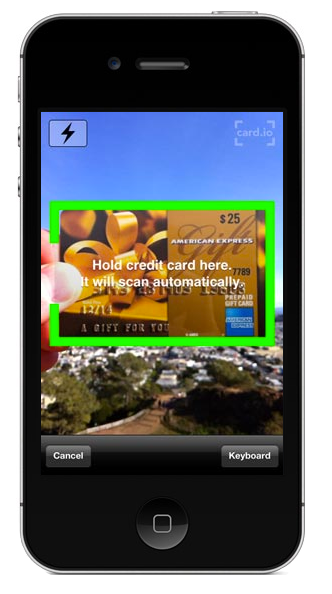
\includegraphics[width=6cm]{cardio}
\caption{Card-io in use sanning a credit card \label{cardioscan}}
\end{figure}



\begin{figure}[ht!]
\centering
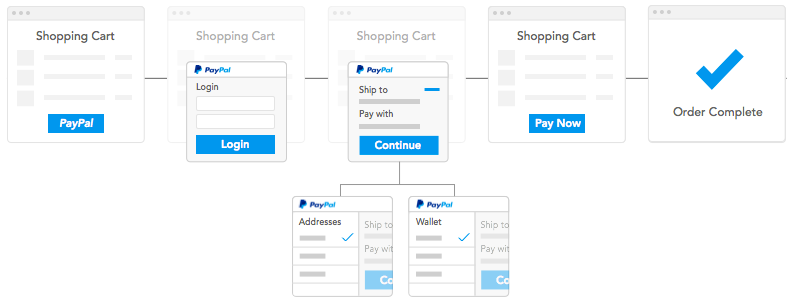
\includegraphics[width=15cm]{vzero}
\caption{PayPal's V.Zero Generic Application Flow \label{vzeroflow}}
\end{figure}

This demonstrates the commercialisation of Douglas' ideas, but this is not the only evolution of reuse, specifically for the personal code reuse of the small-scale developer demographic. However, comparatively less literature has been published and few research efforts made regarding such a demographic, as noted by \cite{Norton2003a} and \cite{Hsieh2006}. The majority of literature refers to large software organisations, but there is considerable need for personal code reuse as well. Norton notes that the majority of small-scale reuse is ad hoc and unstructured, whereas structuring such reuse would enable the developer to become much more efficient with their reuse, and so improve the benefits of engaging with it. The history of such personal reuse, therefore, is difficult to research, but Norton and Min-Sheng both note that there is no obvious practice or standard in place, unlike component-based software engineering.

Therefore, it is clear that code reuse remains a popular concept, and one which can be, and is, employed in multiple ways, dependent on individual ideals; from Douglas' ideas on industrialisation of software development to the current day company repository and work methods, code reuse is ever popular. 

However, small-scale code reuse has been given far less attention, despite it being applicable for individuals throughout their careers, and specifically those that work in relative isolation, such as students, hobbyists, consultants or freelancers \cite{Norton2003a}. Therefore, in the next section, we turn to industry, to seek and analyse potential tools these developers could use that have been built as products instead of research, as well as those available for larger organisations and the industry as a whole.

\section{What tools are there currently that attempt to partially or completely fulfil the goal of cross project, multi user code reuse?}
In this section we will take a look at existing technologies related to the problem domain and analyse their functionality. At the end of the section, we list a set of features these tools may possess, related to fulfilling the original problem description set out in chapter 2, and examine how completely the tools fulfil these requirements.

The technologies below were chosen for a number of reasons, including the author's knowledge of the industry and code reuse, google searches for code reuse tools and similar keywords, and popular technologies. For example, git and GitHub are industry-standard project repositories and implement sophisticated version control and project management tools, so git was chosen based on its widespread use and popularity.

In contrast, Snipplr was found from a search on google using key words “code snippet reuse tool”, and was selected on its immediate similarity to the author's suspected final solution, however, further analysis would reveal that several key features are missing. Finally, the author of this dissertation has experience with several of the tools listed, such as Stack Overflow, and so these tools were included as potential solutions in need of further analysis.

The technologies are presented in ascending order of the author's perceived 'fit for solution', beginning with those which least fit the author's imagined ideal solution. This ideal solution draws from a number of aspects, including the author's personal experience with code reuse, the literature discussed earlier within this chapter and in hindsight of the below complete analysis of the listed technologies. We begin with a minimalist code paste tool, Codepad.org.

\textbf{A} - \textit{Codepad.org} is an online compiler/interpreter that has paste dump capabilities. It allows users to type or paste code from one of 12 languages in to a multiline text box, and then it runs that code and outputs a short URL containing both the source code and any runtime output, which can then be shared by the end user. It is a minimalist code share tool, where source can be saved as 'pastes', and shared via URL. There is little other functionality, other than the ability to make a paste private or save a paste to your account.

\textbf{B} - \textit{Pastebin.com} is similar to Codepad, in that it facilitates 'copy paste' code sharing via a short URL, but does not run the code. It was created in 2002, but was not a popular platform until 2010, when it had achieved 1 million 'active' pastes \cite{Kumparak2011}. In June 2015 this number was more than 65 million active pastes. Pastebin contains more options than Codepad such as language specific syntax highlighting, paste expiration settings, public or private pastes as well as giving it a title, but again does not expand further than simply 'code paste' sharing. Pastebin also exposes an API to allow other tools to utilise its method of sharing, though most seem to be browser plugins. These can be seen on the pastebin website, under tools.

\textbf{C} - \textit{Google Docs} allows users to create and edit documents online, including text documents, spreadsheets, slideshows and forms. It originated when Google acquired Upstartle in 2006 and through 2007 merged their web-based word processor with Google Spreadsheets \cite{Mazzon2006}. While not specific to code, it boasts good online, collaborative features for editing documents, as well as cloud storage, and the ability to make documents private, public shareable or public editable. It also includes version history and roll backs for version control. Despite these features, it is not designed for code storage or retrieval. Retrieving code from the storage would quickly become cumbersome as no efficient categorisation or search tools are present, and performance is on par with NTFS. Therefore, Google Docs' main appeal is real time collaboration and version control of documents.

\textbf{D} - \textit{Stack Overflow} is a language-independent, collaboratively edited question and answer website, and contains a vast wealth of knowledge, and often examples too. It began in 2008 as a website dedicated to helping users seek assistance on programming related issues. Soon after in 2009, additional websites were created along the same premise, under the Stack Exchange umbrella. Within Stack Overflow, questions and answers are voted up and down, and edited in the same fashion as a wiki. Reputation is gained or lost from these votes, resulting in self-policing and consistent high quality content. These features relate to the problem domain as they help reduce stale code, and provide peer review for code snippets. They also allow editing of answers as programming languages evolve and standards change, which is something a static repository often fails to achieve. However, as it is a question and answer website, code sharing is reactive, and usually occurs as an example within an answer. It most certainly does not act as an adequate repository, despite its many usability and collaborative features. Despite this, it is worth noting for its usability features, as discussed.

\textbf{E} - \textit{Integrated Development Environments} (IDE) may come with snippet tools. Sublime and Atom are both text editors for code and markup that include some form of snippet repository within them. These are offline, personal repositories, but the specific files can be zipped and sent to others, albeit with effort from both parties. The snippets are written and stored as files with some form of markup, for example XML. This then allows them to be named, and recalled simply by writing the name of the snippet. For code that is used often, this is a fast and efficient way to reuse code, but requires the developer remember both what snippets are available, and what name they all go by. Searching the repository is often cumbersome, and redundancy is quite possible, as snippets may go forgotten. As it is an offline, personal repository, the problems relating to stale code and lack of peer review remain.

IDE Plugins are also an option, such as Resharper for Visual Studio. Its aim is to improve upon Visual Studio's snippets, though works in quite the same way as the IDE snippet tools mentioned above. Resharper however, can also predict which snippets you may want from the context of your code, among other things. Despite this functionality, it again is an offline, personal repository and maintains the same problems mentioned above that befall the IDE solutions.

\textbf{F} - \textit{git} is a version control software, storing revisions of software in a distributed revision control system, and is widely used in the software development industry \cite{Skerrett2014}. Users can create a repository which maintains a complete history and full version-tracking of itself. This repository can then be cloned to another location to be worked on, and this second repository also maintains a complete history and full version-tracking. Commits can then be pushed between repositories, and changes are merged to allow for seamless collaboration even on the same files. However, git repositories mirror that of a file system, and as such have no real search or sort methods to allow for quick navigation through code snippets. Instead they are used to track source code for individual projects. This would make it cumbersome to use, and although it improves on Google Docs, as it is code oriented, it does not satisfy the ease of access nature that a code reuse repository would require.

\textbf{G} - \textit{GitHub's Gists} initially look very similar to pastebin and codepad, in that the user may type or paste a snippet of code into a textarea, giving it a title, description and privacy options, and then share it via a URL with other users. However, once created, they are treated as a git repository, and can be cloned, revised and added to. This means they act as a combined pastebin and git, bringing with it the benefits of both, however this solution does not improve on the negative points mentioned above for either, and so again would not be suitable as a solution to the problem at hand.

\textbf{H} - \textit{Codebase} is an online repository hosting service that works with git and other similar repository services, but with project tracking features on top. Similarly, Codebase is used to track source code for individual projects, and also handles a number of other project management features, such as tickets, bug tracking, time tracking, customisable permissions, AGILE development and more. A number of these features would be useful in our ideal solution, however again Codebase falls short as it is cumbersome to extract snippets from a repository built in this manner. 

\textbf{I} - \textit{Snipplr} is an online snippet sharing website, and comes close to solving the problem. Users can create public or private (personal) snippets, containing a title, description, source code and other meta data, and save them to their own snippet library. If public, other users can comment on these snippets, favourite them or share them on social media. Snipplr has a number of search filters, including searching all snippets or just personal snippets, searching titles and descriptions, searching source or for specific tags. However, the search functionality is particularly verbose, and only allows for searching one of these filters at any time. Combination search is impossible, so complex filters cannot be created.
Users have profiles, and can gain points and achievements for their snippets through community recognition, in a similar fashion to StackOverflow, and high scoring snippets are more visible to the community. Users also can edit their own profiles to provide personal information about themselves.

At first look Snipplr seems to fit the bill for our problem domain, but a number of features are lacking. There is no version control or snapshot history for code snippets, and by extension there is no tracking information other than time and user of last edit. Additionally, Snipplr has no functionality geared towards sharing within a company or institution. If a company, such as a web development agency, wished to track reusable snippets and provide access to a list of employees, there is no process to do this with Snipplr. Similarly, if an educational institution wished to share code snippets with a specific subset of students, Snipplr would be unable to handle this request. Therefore, a comparison of these core features are necessary, to find which, if any, are most suited as our solution.

\section{What core features can we draw from these tools for our ideal solution?}
From the above break down of these technologies, we can establish preliminary criteria drawn from these tools that we believe would benefit the small scale code reusers. These criteria also allow us to both compare the tools with each other, and begin to conceptualise an ideal overall tool that consists of these criteria. Finally, it allows us to see if any one technology already fits in to this ideal overall tool, or how closely any one technology comes.

Table \ref{corefeatures}. culminates this information, with the individual technologies along the top and the criteria on the left. If the technology implements the criterion listed, a checkmark is placed in the corresponding box.

Before displaying the table, it is useful to explain the chosen criteria, to help give an understanding and greater depth to each criterion. The following bulleted list details this information:

\begin{itemize}
\item \textit{Paste Dump} - Some functionality specifically designed to allow writing or pasting code into a multiline text field, and the ability to find that code again via a URL. 
\item \textit{Exposed API} - An API that enables some or all of the technology to function through third party code, such as calling savePaste(string) or getPaste(id) for a paste dump.
\item \textit{Publicity Settings} - Some functionality that enables some or all of a user's input to be set to public or private. See Grouping Privacy criterion for explicit settings.
\item \textit{Openly Collaborative} - The technology provides the ability for multiple users to collaborate on a single, shared input to the technology. 
\item \textit{Online} - The tool can be accessed over the web, independent of device. Does not exclude the possibility of the tool also functioning offline.
\item \textit{Peer Review} - The ability for other users to view and comment on a piece of code. Functionality could be extended to allow for change requests to be sent, or actual changes to be made by users.
\item \textit{Advanced Search/Sort} - The technology provides advanced search and sort capabilities, including complex filters and search terms such as wildcards, to build a complete search term. 
\item \textit{Version Control} - The technology has some form of version control, including a revision history, accountability tracking and the ability to access the previous versions of the code. 
\item \textit{Grouping Privacy} - The technology provides features that allow groups of people to be defined, and for those groups to be given access to specific portions of the stored code, such as an institution giving private code to its members.
\item \textit{Personal Repository} - The technology provides a personal repository for the users, such as an individual area with space for the user to store what they desire.
\item \textit{Not project focused} - The technology does not focus on projects or project management, and instead remains more abstract.
\item \textit{Snippet Meta Data} - Inputs can be attributed with meta data, such as title, description, search tags, etc.
\item \textit{Synchronisation across devices} - The inputs are synchronised across devices, so changes made on one system are reflected on the others.
\item \textit{Accountability} - Any input, be it an addition, change or deletion, can be attributed to a user, and no such action can be performed anonymously.
\end{itemize}

These criteria were chosen from the set of core features implemented by the previously mentioned technologies, and were selected due to their likely utility within a final code reuse tool. The table below summarises these tools based on these criteria, and we shall use this as our main comparison between the tools. The letters and their corresponding technologies are repeated beneath the table for clarity.


\begin{table}[H]
\centering
\caption{Comparison of core features between existing technologies \label{corefeatures}}

\begin{tabular}{|l|*{9}{c|}}
\hline
                                     & A & B & C & D & E & F & G & H & I \\ \hline
Paste Dump                 & \ding{51} & \ding{51} & & & & & \ding{51} & & \\ \hline
Exposed API                & & \ding{51} & \ding{51} & \ding{51} & \ding{51} & \ding{51} & \ding{51} & \ding{51} & \ding{51} \\ \hline
Publicity Settings          & \ding{51} & \ding{51} & \ding{51} & &  & \ding{51} & \ding{51} & \ding{51} & \ding{51} \\ \hline
Openly Collaborative    & &  & \ding{51} & \ding{51} &  & \ding{51} & \ding{51} & \ding{51} & \ding{51} \\ \hline
Online & \ding{51}     	  & \ding{51} & \ding{51} & \ding{51} &  & \ding{51} & \ding{51} & \ding{51} & \ding{51} \\ \hline
Peer Review                 & & & & \ding{51} & & \ding{51} & \ding{51} & \ding{51} & \ding{51} \\ \hline
Advanced Search/Sort & & & & \ding{51} & & & & & \\ \hline
Version Control            & & & \ding{51} & \ding{51} & \ding{51} & \ding{51} & \ding{51} & \ding{51} & \\ \hline
Grouping Privacy         & & & \ding{51} & & & \ding{51} & & \ding{51} & \\ \hline
Personal Repository    & & & \ding{51} & & \ding{51} & \ding{51} & \ding{51} & \ding{51} & \ding{51} \\ \hline
Not Project Focused    & \ding{51} & \ding{51} & \ding{51} & \ding{51} & \ding{51} & & & & \ding{51} \\ \hline
Snippet Meta Data       & & \ding{51} & & \ding{51} & \ding{51} & \ding{51} & \ding{51} & \ding{51} & \ding{51} \\ \hline
Sync Across Devices   & \ding{51} & \ding{51} & \ding{51} & \ding{51} & & \ding{51} &  & \ding{51} & \ding{51} \\ \hline 
Accountability              &    &    &    & \ding{51} &     & \ding{51}  &      & \ding{51} & \ding{51} \\ \hline \hline
\textbf{Total Checks}   & 5 & 7 & 9 & 10            & 5  & 11            & 10 & 10           & 10 \\ \hline
\end{tabular}
\end{table}

\begin{enumerate}[label=\Alph*]
\item - \textit{Codepad}
\item - \textit{Pastebin}
\item - \textit{Google Docs}
\item - \textit{Stack Overflow}
\item - \textit{IDE \& Plugins}
\item - \textit{git}
\item - \textit{GitHub Gists}
\item - \textit{Codebase}
\item - \textit{Snipplr}
\end{enumerate}


These criteria are necessary in order to evaluate and compare the systems, but they will also provide a base from which to advance future research from, specifically in the next chapter when we question current industry experts for their habits and ideals behind code reuse at this scale. 

The criteria table shows us a number of important facts, as well as which technologies stand out as most matching our ideal set of criteria. We can see that codepad and pastebin are part of only three technologies that incorporate a paste dump, and that Gists is the only tool that acts further upon these paste dumps, turning them into repositories of their own to be worked on further. We also see that being \textit{Online} and having an \textit{Exposed API} are common attributes, appearing in all but one of the technologies. This would suggest that online tools are preferred, either by the developers to build or the users to utilise, though this may also be due in part to the research methods utilised and so needs further research to fully justify the reasoning.

It is clear that the paste dump services and the IDE \& Plugins do not facilitate the role of a code reuse repository akin to the likes we are looking for. They each meet half or less of the criteria, and implement no advanced features (such as version control or advanced search/sort). However, their functionality is not implemented by the majority of the other technologies. This makes them worth reviewing as we will need to analyse whether that functionality is necessary in our final application, why other technologies haven't replicated the functionality, and whether their API is worth using instead if that functionality is required. We can see that GitHub's Gist ties in their paste dump service with the other features, and so this will be the system we analyse further when we look to develop or implement paste dump functionality.

\textit{Publicity settings and Snippet Meta Data} are two more features commonly seen throughout our chosen technologies. Each were seen in seven of the nine technologies, suggesting they are also key features of the technology. Publicity settings did not appear in the IDE \& Plugins or on Stack Overflow, though this is likely due to the nature of the two technologies - the IDE \& Plugins were offline and specifically designed for one person, so would not need publicity settings, and Stack Overflow, being a collaborative Q\&A system, would not function with publicity settings. It would, however, be possible for Stack Overflow to implement a group privacy setting to restrict certain questions from only being answered by set groups, though this is not something I witnessed.

\textit{Group privacy}, instead, is implemented by a subset of the technologies which implemented publicity settings, by only Google Docs, git, Gists and Codebase. The author of this dissertation feels this feature is important when considering functionality of the envisioned system, as it would allow for groups or institutions to utilise the technology and restrict access to only its members. This feature is one of several which Snipplr do not implement, along with version control and advanced searching and sorting, which are key reasons why Snipplr does not fully encompass the expected outcome deliverable of this dissertation.

Of these final other features, \textit{Version Control} is the more common, being seen in 6 of the technologies, however, advanced searching and sorting can only be found in Stack Overflow. For a repository, being able to search for complex terms and filters efficiently is a key requirement to facilitate the reuse of deposited code, and aid the user in finding code they may not know exists within the repository. This is because users of the repository must be able to find and reuse components faster and easier than writing the code from scratch \cite{Krueger1992}. 

Human beings are utility-maximizers \cite{Cognition1997} - that is to say, they seek the approach that yields more value than its cost, meaning code reuse will only be embraced when it is believed that reusing the code is easier than writing it themselves. Users may remember a piece of code, but not when or for what they developed it, which makes finding and reusing the code difficult or more cumbersome. A reuse repository requires that finding and reusing the code be more efficient than simply rewriting it, which in turn requires that searching the repository be fast and efficient. If one must spend 10 minutes recalling the code, and another 10 searching for it, when it could have been written in 15 minutes, the repository is not fit for purpose and instead negatively impacts the developer. To this end, advanced searching and sorting is a key component of the ideal solution, and therefore, the technologies that do not implement this feature are far less likely to fully encompass the requirements of our expected deliverable. Consequently, we shall focus on Stack Overflow when we research further into advanced search and sorting, to identify how it should be implemented in the final deliverable.

We have discussed the core features of these technologies and explained the reasons behind why they are important. This has shown that no single technology fully encompasses these requirements despite their relevancy in the final deliverable, and would suggest that the final deliverable itself will be a new technology, built from the core criteria researched above.

Having established these core criteria for our system, we can now begin to look at optional features that the existing technologies implement - usability features that aren't necessary for full functionality, but that improve the day to day usage of these specific tools. In the next section, we discuss the most prominent usability features pulled from our set of technologies, and evaluate how each tool improves the quality of the software and its use.

\section{What usability features do these tools implement and utilise?}
The discussed technologies implement a large array of usability features, ranging from user interface additions or backend functionality, to user-to-user interaction or organisation tools. For this reason, noteworthy features have been extracted from the technologies and grouped in to categories, then given a brief description to aid understanding. The categories were chosen by the author in an attempt to encompass fully the selected optional features, and provide a logical categorising for analysis.

\begin{itemize} 
	\item User Interface
	\begin{itemize} 
		\item Markdown for description or comments
		\begin{itemize}
			\item Utilises plain text formatting syntax to mark-up text, to be easily translated into HTML and other formats for display. \cite{Markdown2004}
		\end{itemize}
		\item WYSIWYG Text Editor
		\begin{itemize}
			\item What You See Is What You Get - allows the developer to see what the end result will look like while the source is being written \cite{Oxfordnd}, such as when HTML or Markdown is included in the text.
		\end{itemize}
		\item Syntax Highlighting
		\begin{itemize}
			\item Changes the colour of text, usually source code, according to a catalogue of terms or a language syntax, such that the readability is improved.
		\end{itemize}
	\end{itemize}

	\item User-to-User Interaction
	\begin{itemize}
		\item Rate, Pin/Favourite, Comment, Share
		\begin{itemize}
			\item Ratings allow users to express their opinions quickly and show the aggregate opinions of fellow users, for example through a 5 star rating, or by giving users the ability to +1 or -1 the score of a submission.
			\item Pining or Favouriting is the act of a user expressing their want to return to the submission for future use by storing it in a special, personal list.
			\item Commenting goes further than rating, by giving the user a way to express their opinion verbatim, and culture discussion around a submission.
			\item Sharing allows users to bring others into the fold by distributing the submission, through social media or more conventional methods such as email.

		\end{itemize}
		\item Profile - information about the user, their submitted code and more
		\begin{itemize}
			\item The profile allows a user to find out more about other users, or look at other user's submissions to the technology.
		\end{itemize}
		\item Achievements
		\begin{itemize}
			\item Achievements are a method of gamification \cite{Huotari2012} for a technology, and promote user activity through unlocking rewards for completing tasks.
		\end{itemize}
		\item Report Submissions
		\begin{itemize}
			\item This allows for a community to self-police itself, and ensure unwanted or spammy posts are removed with less or minimal effort.
		\end{itemize}
	\end{itemize}

	\item Content Navigation
	\begin{itemize}
		\item Tagging, Indexing, Searching/Sorting
		\begin{itemize}
			\item Tagging allows users to add specific meta data to submissions to aid future search and sorting. This could involve describing the type of submission, where or when it was written, or what language it's in, and is commonly seen as a list of key words. 
		\end{itemize}
		\item User groups/companies/institutions
		\begin{itemize}
			\item The technology enables users to create groups and invite other users in to them. They may have a hierarchy of admins and members, or have all users be equivalent, and can be used by companies or institutions to distribute submissions to all of its members.
		\end{itemize}
		\item Public/Private snippets/groups
		\begin{itemize}
			\item The ability to mark a submissions as public or private, or add a list of users that are able to view the submission, either individually or as a group.
		\end{itemize}
		\item Forks/Change Requests/Branches
		\begin{itemize}
			\item Users are able to take a copy of a submission and change it, potentially submitting their own, or requesting that the original one be merged or replaced with their updated version.
		\end{itemize}
		\item Related submission
		\begin{itemize}
			\item The technology provides quick access to related submissions that the reader may be interested in viewing or using.
		\end{itemize}
		\item Submission Grouping/Multi-part Submission
		\begin{itemize}
			\item The ability to create submissions that are part of a small collective of submissions, and as such are linked together by some method.
			\item For example, a submission may be for template code for a dynamic button on a website. One part utilises HTML for markup, another uses CSS for styling and a third part incorporates JavaScript for animation.
		\end{itemize}
		\item Custom groups for submissions
		\begin{itemize}
			\item Predefined or User-created groups for submissions, such as collecting snippets used in web development, those used in software development, and design documents all into different groups for ease of access.
		\end{itemize}
		\item Cloud Storage/Computing
		\begin{itemize}
			\item Cloud Computing refers to on-demand network access to a set of resources, often utilised as programs that don't need to be downloaded, installed or run on the local system \cite{Anjomshoaa2011}.
			\item Cloud Storage refers to data being stored across multiple servers or locations, with the digital representation of this data exists in a single access point for use, such as on one website.
			\item This allows for applications to be used immediately, from any host, without any prerequisite short of internet access and some medium, such as a browser, making it highly accessible.
		\end{itemize}
	\end{itemize}

	\item Third party tools

	\begin{itemize} 
		\item Integrated Development Environment (IDE) Integration via API
		\begin{itemize}
			\item Snippets saved to the technology can be accessed from within the IDE via exposed hooks to the technology. Might include user authentication.
		\end{itemize}
		\item Facebook Login for easy account creation/future login
		\begin{itemize}
			\item Utilising exposed account APIs via OAuth protocols, user details can be passed from Facebook to the technology to facilitate account creation and login.
		\end{itemize}
		\item Social Media integration for sharing code
		\begin{itemize}
			\item Exposed API from social media allows code to be shared on those social media, such as Tweets on Twitter or Facebook messages.
		\end{itemize}
		\item WordPress Plugin
		\begin{itemize}
			\item Similar to social media integration, a WordPress plugin would allow functionality from the website to be utilised by the WordPress platform, and as such, by websites running WordPress.
		\end{itemize}
	\end{itemize}
\end{itemize}

These usability features are all optional for a final system, but each one can be useful for specific use cases or certain user bases. For example, \textit{Third Party Tools} enable the technology to fit more easily in to a user's workflow, or create a more seamless integration for utilising the tool, including before, during and after development, such as planning, developing and sharing. \textit{User Interface} additions help make the technology more accessible, efficient or easier to use, and can help users quickly understand how to use the technology, or make sense of a submission, such as with Syntax Highlighting.

\textit{User-to-user interaction} is important to promote a social environment within the technology, while also enabling users to more easily engage in cross-user interaction. User interaction facilitates two of the core features, collaboration and peer review, and as such, these optional features play an important role in the final system. Finally, \textit{Content Navigation} makes up a large bulk of the optional features, which is to be expected, as the technology will be responsible for storing, categorising and retrieving content in the form of submissions and as such, these features will focus heavily throughout the technology.

The next step for the optional features is to describe their priority relative to each other. In the next chapter, we delve into this task, and present opinions collected from an array of end users, including industry professionals from a range of companies, and undergraduate students studying Computer Science. Ultimately, we intend to finalise the requirements for the deliverable.

\section{Conclusions}
As stated at the start of this chapter, our goal throughout this section was to determine whether the problem domain of small scale code reuse has been sufficiently explored, and whether there are adequate technologies currently that address the domain. We explored the history of code reuse, from its roots up to its modern day evolution, and discovered that, although papers on reuse are not uncommon, those focused on individual or small scale reuse are sparse, and this has been noted in several published works.

We also described nine potential technologies, and investigated how they work and what they accomplish. From this we identified fourteen core criteria that our desired system should facilitate. Unfortunately, none of the technologies managed to fully encompass all these requirements, which suggested that technology, like the literature, does not provide adequate coverage for users of small scale code reuse. 

Further to the core features, we identified many optional features that promote user experience. These were aggregated from the technologies we described, and will be used in practical research to help mould the deliverable we intend to create. This practical research will be conducted with the help of professionals from multiple industries, and students in educational institutions. We will utilise their input and knowledge from their own code reuse experiences, and collaborate their feedback and opinions into the requirements and design phase throughout the next chapter.

To conclude, we feel there has not been adequate research in to small scale code reuse, nor is there a sufficient technology able to fully address the needs of the code reuser. We intend to design, construct and evaluate such a technology in an open source environment, with the desire of improving small scale, cross project code reuse. The first step for this begins in our next chapter: the requirements and design for such a system.




%% Chapter for the Requirements and Design
\chapter{Requirements \& Design}
%% If you are doing a primarily software development project, this is the 
%% chapter in which you review the requirements decisions and
%% critique the requirements process. Then, you review your design decisions at various
%% levels and critique the design process.

\section{Introduction}
Throughout this chapter, we detail the requirements for our system, both functional and non-functional, by drawing on the core and optional features described in the previous chapter. With these in mind, we then move on to consider the design of our proposed deliverable, and set specific goals for it, which will later be used as measurements of evaluation for the system.

\section{Requirements}
We begin by translating the previous core features in to functional and non-functional requirements, 



%% Chapter for the Implementation and Testing
\chapter{Implementation}
%% & Testing
%% This is the chapter in which you review the implementation and testing
%% decisions and issues, and critique these processes.

\newlist{requirementsrevisit}{enumerate}{1}
\setlist[requirementsrevisit]{label=\textbf{R\arabic{subsection}.\arabic*}}

\section{Introduction}
Throughout this chapter, we divulge and explain the third party software and toolset we used to implement the system.
We also look to describe problems faced along the way, and the proposed solutions to those problems. 
It is important to notice that not all issues are included: trivial or academically uninteresting problems are ignored in favour of those more interesting and relevant. 
An assumption is made that the reader has a working knowledge of web development throughout this chapter.


\section{Base Technologies}
\subsection{Clientside Technologies}
In section \ref{littechconclusion}, it was decided that the system should be a website based application, and we desire it so that users can access the system independent of browser, operating system or device.
It was felt that developing and testing for the top three most used browsers, as reported by w3schools.com (http://www.w3schools.com/browsers/browsers\_stats.asp) would cover adequate scope for the timeline of this project, and further browser testing and tweaking will be left for future work. 
Thus, the browsers chosen were Google Chrome, Firefox and Safari.

In order to achieve this browser-agnostic system, we built the website using standard web technologies, specifically HTML5, CSS3 and JavaScript.
These languages enable a page to provide content, styling and interaction, respectively.
The goal was to ensure that the code would work well across browsers and operating systems, with small, trivial adaptations applied in specific circumstances.
Due to limited time for this project, it was decided to focus on the release of each browser with the highest percentage of users in the month that testing began (February 2016), as reported by w3schools.com (http://www.w3schools.com/browsers/browsers\_stats.asp). 
This amounted to the versions C48 for Google Chrome, FF 44 for Firefox and S 9 for Safari.
The system was also developed to run on an iPad and iPhone, to get as close to a device-agnostic system as time and resources allowed. Further devices are left to future work.

Further to this, all code was run through the W3C compliant check to ensure the code is compliant with web standards.
Having standardised code provides a degree of confidence that the website will function correctly as browsers update, or in different browsers not yet tested.

All of this together resulted in a base system that users can visit and navigate, though no interaction was possible, due to no memory or state change within the system.
In order to achieve this, database and serverside technologies are required, to communicate between the database, the web server and the client's browser, providing the degree of state change we require.
Figure \ref{homepage} shows the design of the homepage, with placeholder data, which will later be served by the serverside technologies.

\begin{figure}[htb!]
  \centering
  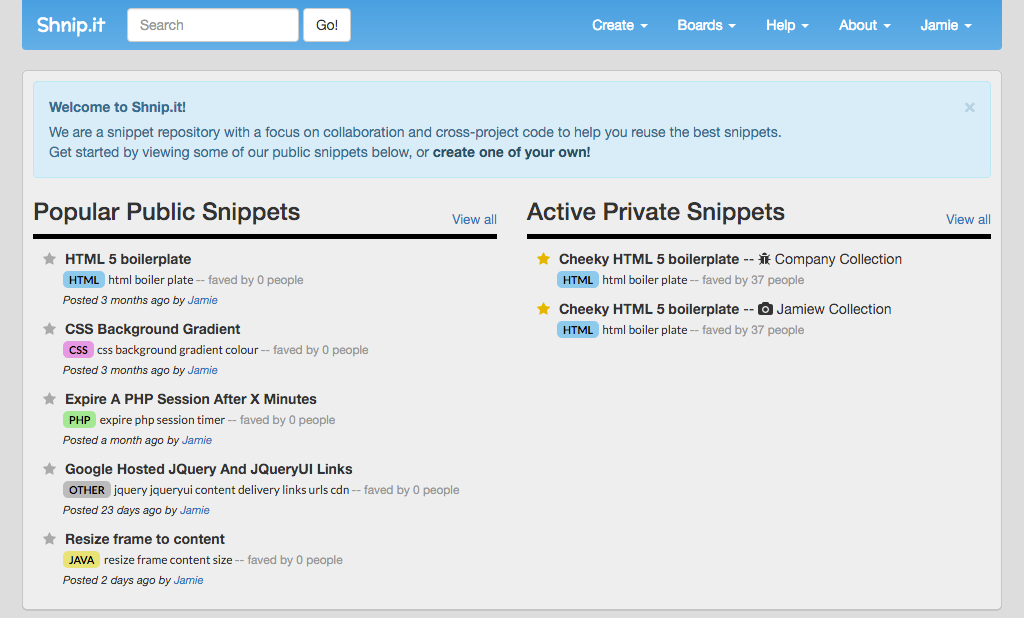
\includegraphics[scale=0.4]{homepage}
  \caption{Shnip.It's Home Page \label{homepage}}
\end{figure}

\subsection{Serverside Technologies}
The chosen technologies for the serverside are PHP and MYSQL, due in part to the authors experience with them, and the fact that, as a pair, they are well known in industry.
PHP is parsed before the webpage is sent to the client, and the output of any PHP process is plain HTML that can then be sent to the web browser for viewing.
This provides an efficient method of querying the database to retrieve information depending on which page the user wished to view, and then providing that page with the appropriate content filled in via PHP.
PHP is also used to handle the majority of website functionality, including account registering/login, the editing and saving of snippets, and all other information related to the usage of the website.

We also use a MYSQL database as it provides a relational structure suited to the envisioned structure of the website. 
The interaction between PHP and MYSQL is well-structured and documented, allowing for easier development of the website's backend.
Finally, a visual representation of the database is provided via a tool named PHPMYADMIN, which is accessible from the server's IP, as seen in Figure \ref{phpmyadmin}.
This technology is useful for quickly creating the database, and managing it visually.

\begin{figure}[htb!]
  \centering
  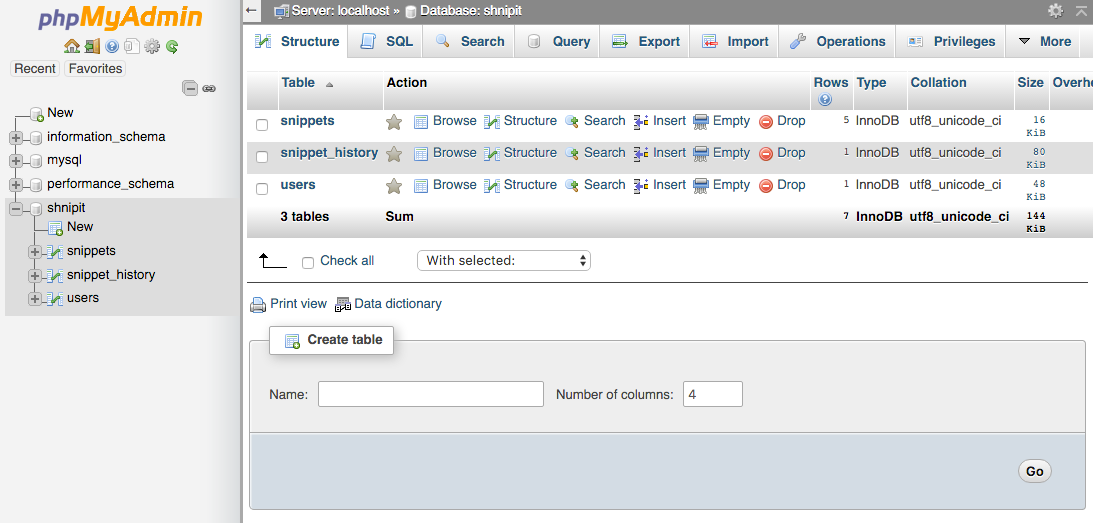
\includegraphics[scale=0.3]{phpmyadmin}
  \caption{Shnip It database structure, visualised in PHPMYADMIN \label{phpmyadmin}}
\end{figure}

\section{External Plugins \& Libraries}
\subsection{Environment Libraries}
A number of external plugins were utilised within the development environment, either as a way to write better code or to promote the cross-compatibility of the code across browsers.
The first of these technologies was named SASS, and the second, its counterpart Compass. 

SASS is a precursor language that converts its markup into valid CSS, while providing the user with functionality not available with standard CSS.
Such functionality includes variables, for example hexidecimal colour codes, that can be reused throughout the SASS and easily changed, or mixins that allow code to be written once and reused throughout. 
This enables a more object oriented style of CSS to be written, and cuts down on development time, both initially and in the future when the design may change.
Furthermore, Compass is used as a utility that converts these SASS files to CSS files on the fly, and allows the developer to forget about the conversion process.

Finally, a stylesheet named Normalise.css was utilised which resets a number of styles that may differ by default between different browsers, for example margins or padding on specific elements.
It was used to give a more consistent baseline between browsers, so that less minor tweaks were required further down the line.

\subsection{Development Libraries}
A number of development libraries were used, either to provide functionality that had already been created, or to use as a method of writing less code.

Bootstrap is the first library used; it offers a styling baseline for the website, including dynamic grids that can adjust easily to screen size, certain pre-created elements such as notifications, widgets and buttons, and a general, good practice environment from which to build upon.

JQuery was utilised to make page-specific Javascript easier to perform. 
The design involved interaction between the user and the page, such as rating a snippet or submitting a comment; as such, jQuery allowed for more effective and efficient interaction, by providing immediate confirmation of a successful action, as opposed to refreshing the page to show the updated content.
Examples of these are showing the comment on screen, or colouring in an up arrow for a positive rating. 

Finally, we used a number of libraries that had been created to do specific tasks, rather than re-writing them. 
This included Prism to handle the syntax highlighting, an optional feature noted in section \ref{optionalfeatures}, Moment maker to make `fuzzy timestamps' such as 3 hours ago, and identicon to create unique default profile pictures based on a user-centric alphanumeric string. 
All 3 of these libraries can be seen in Figure \ref{snippetpage}.
These are all libraries to handle optional features that were included in the final system.

\begin{figure}[htb!]
  \centering
  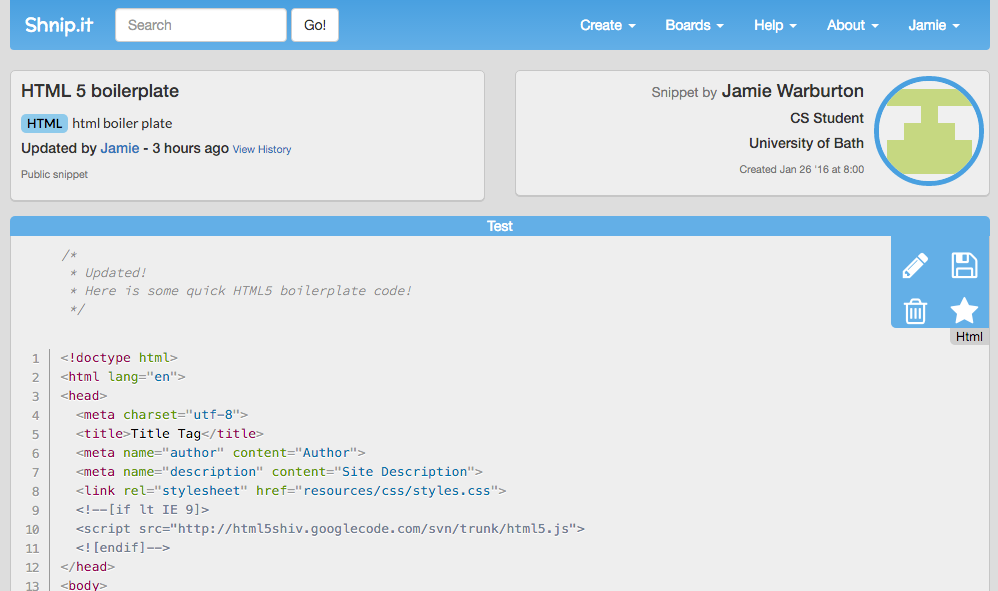
\includegraphics[scale=0.4]{snippetpage}
  \caption{Snippet Page - Syntax Highlighting, and `3 hours ago' fuzzy timestamp \& Identicon \label{snippetpage}}
\end{figure}

\section{Novel Problems}

\subsection{Database Design and Access}

A key component of our system was the database, as it would hold the entire catalogue of the website; without it the website would not function.
This meant it was important to design it to be efficient, robust and secure. 

\subsubsection{Designing the Database}
Due to the nature of how accounts and snippets are linked, a decision was made to build a relational database, enabling a table per element, and to link them via IDs.
However, this posed two novel problems - how would we calculate, store and retrieve the number of upvotes and downvotes a specific post has received - and by whom - and also how to handle the version history and control of snippets, specifically in relation to snippet collections.

\subsubsection{Upvotes and Downvotes}
There are two obvious approaches to this problem: \\
	1. Create a table for upvotes and downvotes, and attribute each vote to a snippet ID, and a user ID, and calculate the total when required, or \\
	2. Ignore the normalisation of the database, and just store a total in the snippet table for each snippet, and increment or decrement as required.

Both of these methods suffer from some form of scalability issue. 
For the first approach, recalculating would have to be performed every time the value of the total number of votes was required, which can equate to several times per page refresh, or many tens of times per homepage refresh, due to these pages showing information for more than one snippet.
Multiplied by the number of users active and this can become quite the computationally expensive solution.

The second method opts to store the total in the table with the snippet, and so cuts out a significant portion of the computation originally suggested.
However, with this solution, the total can easily fall out of sync with reality, as parallel writes to the database may conflict or not be recorded, and the database may spend a considerable portion of time trying to ensure that increments and decrements were not overwriting each other, and attempting to maintain an accurate record.
In practice, this equates to a slow, inaccurate database. This problem is further compounded by the fact that there is no record of who has voted, and so no method of preventing a user from voting multiple times.

After some research into this issue, it was decided to follow a pattern similar to that of Stack Overflow's, which is a hybrid of the two solutions above. 
Initially, we store a total value within the snippets table, and ignore the normalisation exclusively for this field.
We also keep a separate table consisting of snippet ID, user ID and the vote value (1 or negative 1). 
When we need to display the total value of all votes, we simply query the snippet table and receive the total as listed, which solves our expensive computation problem on reading the total.

Next, when a specific action occurs, such as a user up or down-voting a snippet, the system records the vote in the correct table, then recalculates the total value of that snippet, and updates the snippet table. 
This solution avoids the out-of-sync problems faced, while also providing a record of who has voted, and as reading the total is much more common than writing it, the expensive computation on reading the total is ultimately reduced, and in turn significantly lowering the computational cost of the overall solution.

\subsection{Version History}
The next issue we encountered was related to storing the version history for each snippet in an efficient manner.
At first this does not seem like a trivial problem, however it was confounded by the inclusion of `grouped snippets' - that is, groups of snippets that go together, for example a snippet of HTML, one of CSS and one of JavaScript that collectively describe a button.

Initially we had a single table of all snippets, each having an ID and a date. 
These two fields together allowed us to describe a unique snippet, with all historical versions having the same ID but a different date.

However, this resulted in duplication of static data, such as original author and date of creation, amongst other fields.
To remove this redundant data, a two table design was utilised - one to parent the snippets, which has a single row per snippet, and one to contain the historical data for the snippets.
The two tables were linked by a field named `child snippet', which stored the ID of the historical snippet, and functioned identically to the original design in the previous paragraph.

This worked well until the inclusion of grouped snippets, as a method of tracking the parent snippet, as well as all the children snippets, was required.
A simple solution would have been to create another table of a similar design, which would be the parent of the grouped snippets, and would store the IDs of the static snippets, which in turn hold the IDs of the versioned snippets.
It is easy to see this design is cumbersome and could quickly become a burden, and so a different solution was required.

We already had the static snippet table functioning as a parent for the version history snippets, so felt it was natural to extend this.
We opened up the `child snippet' field to accept an array of IDs, and so it became `child snippets'.
This structure can be seen in Figure \ref{tablelayout}.
Now we were able to track all of the child snippets, but it left us with a number of questions surrounding how to treat each snippet in terms of interaction - should they have their own rating systems, or collectively for the entire snippet group?

\begin{figure}[htb!]
  \centering
  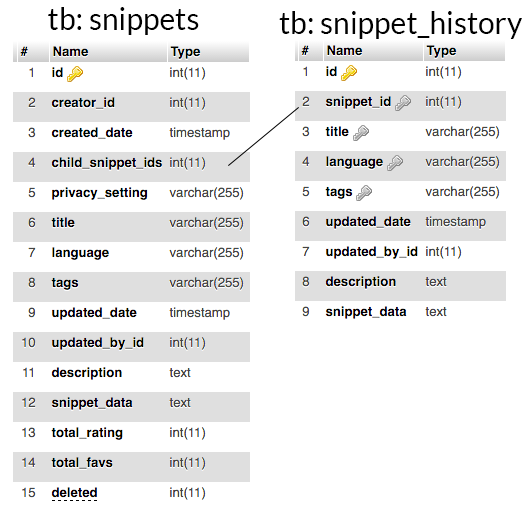
\includegraphics[scale=0.6]{tablelayout}
  \caption{Database Structure - Grouped Snippets \label{tablelayout}}
\end{figure}

For the purpose of this dissertation, each group was treated as a single snippet, and were given a single, overall rating system. We leave it for future work to research and conclude the preferable method for this.

\subsection{Database Security} \label{DBSec}
For the website to function, the database must hold user information and passwords, and therefore must be secure.
It is of great importance to endeavour to follow best practices surrounding this sensitive data and the storage of it, therefore research into this area was required.

We began with the most obvious - account information, and specifically the passwords. 
As we are using PHP, the best practices for password storage were researched, and it was decided to use PHPs built in password hashing functions. 
With this, PHP handles the password hashing and checking, and allows us to simply store the hashed string in our database for later comparison.
As PHP updates, so too do the functions, and as such the system is given an evolving method of security with little cost to development or maintenance.

Next we turned to the security of the database itself. 
Initially the user accounts that login to the database were considered, and these were given complex passwords, particularly for the root users, to help prevent brute force attacks on the database itself.
The user permissions were also cleaned up to ensure only necessary permissions were given to each of the user accounts.

Last on the list was the code. 
Initially we made sure that only the web server had access to any files that contain database login information, so they couldn't simply be found and viewed outside of the web server. 
Then the interaction with the database was examined, via SQL.
This is important due to a method of hacking called SQL injection.
While there exist a number of methods to prevent this, such as prepared statements, it was decided instead to use an external library, called Medoo.

Medoo is a lightweight PHP database framework, built by developers more versed in database design and security than the authors of this dissertation.
Medoo allows us to call simple functions to interact with the database, while maintaining the full security of more complex code, as Medoo wraps this code for us.
The end result is relatively simple interaction code for us to write, without having to worry about security every time we write this code.
A final benefit of Medoo is similar to that of PHP - the code is updated to include any new security features, but our code remains the same, so maintaining the website is less troublesome.
Sample code for inserting data into the database via Medoo can be found in Appendix \ref{medoocode}.


%% What users can access - Groups, private boards, private group boards etc

\section{Summary} \label{implementsummary}

\subsection{Revisiting the Requirements} \label{requirementsrevisited}

We now revisit our list of requirements and discuss how well we have delivered upon them:

\subsection{Delivery on Non-functional Requirements}
\textbf{These Requirements had a high priority}

\begin{requirementsrevisit}

    \item Security \label{security} \\
	\textit{Our system is in line with current best practices, and employs the use of libraries that can easily be updated to incorporate updated security without code changes. Passwords are only stored as hashes via approved methods, private files are only accessible by the web server, and all database user passwords and permissions are set appropriately.}

    \item Ease of Use \label{easeofuse} \\
	\textit{This will be ascertained throughout the course of the evaluation. However, the system has a clear design with obvious icons to indicate functionality and so should be sufficient.}

    \item Simple and Clear \label{simpleandclear} \\
	\textit{This, too, shall be ascertained throughout the evaluation. Again, the clear design and obvious icons should help alleviate mistakes.}

    \item Memorability \label{memorability} \\
	\textit{The simplistic nature of the website combined with the minimal number of pages should allow users to easily re-establish proficiency in use.}

    \item Familiarity \label{familiarity} \\
	\textit{The website uses standard icons for particular functions, as well as obvious styling for elements such as buttons, links and interactive elements.}

    \item Self Policing \label{selfpolicing} \\
	\textit{The system enables users to vote up and down snippets, and uses these votes to automatically police the content via hiding it if it goes too low, and prominently displaying the higher rated snippets. The system also enables users to comment their opinions, and submit edit requests to improve the code.}

Overall we feel our high priority Non-Functional requirements were met well.

\end{requirementsrevisit}

\textbf{These Requirements had a low priority}

\begin{requirementsrevisit}[resume]

    \item Open Source \label{opensource} \\
	\textit{The system currently is not open source, however this is a simple change to make which we leave to future work.}

Overall our low priority Non-Functional requirement was not met, though it is left for future work.

\end{requirementsrevisit}


\subsection{Delivery on Functional Requirements}
\textbf{These Requirements had a high priority}

\begin{requirementsrevisit}

    \item History \label{history} \\
	\textit{The system keeps track of all additions/changes/deletions made, in completion, within the database.}

    \item Accountability \label{accountability} \\
	\textit{The system stores the user ID alongside all additions/changes/deletions to attribute them to that user.}

    \item Social Activity \label{socialactivity} \\
	\textit{The system provides comments, ratings, favouriting and edit requests to allow interaction, both user-to-user and user-to-snippet.}

    \item Content Navigation/Discovery \label{content} \\
	\textit{While a high priority requirement for our system, this is thought to be out of scope for the purposes of this dissertation. Instead, a minimal search function was implemented, to allow users to navigate and discover content, though advanced search is left for future work.}

    \item Privacy \label{privacy} \\
	\textit{The system provides the ability to set snippets to public, private or accessible by a set of email addresses. Accounts with those email addresses attached are then able to view the content.}

    \item Password Security \label{passwordsecurity} \\
	\textit{The system uses PHP's built in functions to hash passwords, and allows these functions to easily update with appropriate advances in the technology.}

    \item Data Security \label{datasecurity} \\
	\textit{All unauthorised material is hidden by a login authentication wall. Some of the website is accessible without an account, but interaction requires login and authentication.}

    \item Platform Compatible \label{platformcompatible} \\
	\textit{The system works appropriately on the latest versions of Google Chrome, FireFox and Safari, on both Windows 7/8/10 and Mac OS X El Capitan. It also works appropriately on iPhone and iPad with Google Chrome and Safari.}

Overall, the majority of our high priority Functional requirements were met, with the exclusion of complex search and sort. However, this requirement was deemed out of the scope of this dissertation, and so was left for future work.

   \end{requirementsrevisit}

\textbf{These Requirements had a low priority}

\begin{requirementsrevisit}[resume]

    \item Gamification \label{gamification} \\
	\textit{The system as of yet does not employ gamification - however we leave it to future work to implement points for positive submissions, and achievements for completing particular milestones, which can be shown on your profile and be made public.}

    \item Submission Groups \label{submissiongroups} \\
	\textit{Snippets can be combined into snippet groups, allowing for multiple snippets to be treated as one singular snippet, for example HTML, CSS and JavaScript snippets that are grouped and describe a singular button.}

While we achieved one of the low priority Functional requirements, we didn't include gamification. It was decided that this will be left for future work, but plans for how to proceed were decided already.

\end{requirementsrevisit}


These will be evaluated further in the evaluation chapter of this dissertation, however, as the majority of the requirements were met, we can expect a satisfactory solution.

\section{Conclusion}
Throughout this chapter it was shown that the implementation of our system has met almost all of the high priority requirements, with the exception of one deemed out of scope of this dissertation. 
We have also discussed novel issues faced throughout the implementation and the solutions chosen to overcome them.
The next chapter describes the user studies we performed to evaluate our system.




\chapter{Evaluation} \label{evaluation}
%%This is the chapter in which you review the outcomes, and
%%critique the outcomes process.  You may include user evaluation here
%%too.
%%
%%Code can be output inline using \verb@\lstinline|some code|@.  For example,
%%this code is inline: \lstinline|public static int example = 0;|  (I have
%%used the character \verb@|@ as a delimiter, but any non-reserved character
%%not in the code text can be used.)
%%
%%Code snippets can be output using the \verb|\begin{lstlisting} ... \end{lstlisting}|
%%environment with the code given in the environment.  For
%%example, consider listing \ref{Example-Code}, below.
%%
%%\begin{lstlisting}[breaklines,breakatwhitespace,caption={Example code},label=Example-Code]
%%public static void main() {
%%
%%  System.out.println("Hello World");
%%
%%}
%%\end{lstlisting}
%%
%%Code listings are produced using the package ``Listings''.  This has many
%%useful options, so have a look at the package documentation for further
%%ideas.

\section{Introduction}
Throughout this chapter we evaluate Shnip It, describing how it meets the original intentions of the system and the studies undertaken to appraise this.

\section{Overview}
As specified in Section 1.2, Shnip It is intended to meet a number of criteria:

\begin{itemize}
\item Provide a system to allow small scale developers to reuse code
\item Provide a method of keeping this code updated with language advancements
\item Provide a method of peer review to increase and maintain code quality
\end{itemize}

We also noted that the system should 
\begin{itemize}
\item Evolve with the needs of software developers. 
\end{itemize}
This last criterion is distinct from the previous points, as it is related to how the system was, and will continue to be, developed, rather than what was actually developed, and so we shall explore this criteria first.

\section{Evolve with needs of developers} \label{evolvewithneeds}
\subsection{Maintaining the Repository}
The key factor in allowing the repository to evolve with the languages is to build it to be both scalable and easily maleable.
The simplest method of doing this is to use plugins and libraries that will be updated with the language itself, without changing the API to use them.
This allows our code to remain the same, but for the actual process and executed code to update appropriately.

As discussed in section \ref{DBSec}, this method was employed for database security, allowing our hashing functions to automatically update, but it has also been used elsewhere within the website, such as for creating identicons, the WYSIWYG code editor and the syntax highlighter for snippets.

Having these plugins removes the need to update the code ourselves, and instead allows us to simply update the plugin files, to keep our software up to date.

\subsection{Evolution of the Repository}
One method of maintaining our repository has been discussed, which is via plugins, but the majority of the website functionality is still written by us, so a method of easing the maintenance and future development of this is required.
It was concluded that the easiest way to achieve this would be to build the system using best practices and object oriented programming - that is, considering future development throughout current development, and ensuring that functionality is modular, so parts can be updated and altered without affecting their functionality and cohesiveness.

This meant that, throughout development, it became paramount to maintain general code where possible, while grouping specific, less-general functionality together, meaning the general code could easily be adapted to include new features, and the specific code could simply be changed in one place when necessary. 
For example, when we pull specific data from the database, such as snippet information, we simply call a function which returns an array of the data we want.
This means, if we were to add an extra field to the snippet data or change it in some manner, we simply need to update one function call to allow it to be used, rather than in all cases where snippet data is collected.
This particular function can be found in Appendix \ref{snippetgrab}.

Similarly, it was important to keep the CSS stylings as general as possible, so that they can be used across the website to maintain styling on all elements, such as keeping buttons or containers the same style with little effort.
This means we can easily change all similar elements across the entire site without complication.

We now move on to look at the remaining 3 criteria, describing the studies we performed and the evaluation methods used.

\section{Evaluative Studies}
\subsection{Approach} \label{approach}
Initially, a usability study was conducted to get a feel for how users will interact with the system, and to discover how it may be improved, before we move on to a quantitative study. 
From this study, we desired to understand how a new user would approach the system, with the key idea being that the user is able to use the system to reuse code, as per our first criteria.
We also use this study to see how users interact with existing snippets, such as submitting an edit request to update a snippet, as per language advancements, and to improve a snippet submitted by another user.
These scenarios are tested to assess the second and third criteria mentioned in the Overview of this chapter. 

These tests are performed in the context of our requirements in section \ref{nonfuncreq}, specifically \ref{easeofuse}, \ref{simpleandclear}, \ref{memorability}, \ref{familiarity} which pertain to how well the user can use the system, both initially and after some time.
\footnote{It is the aim of this dissertation to perform two usability studies, with the second repeated after improvements have been made as a result from the first, but due to time constraints the second usability study is left for future work.
This also means we cannot test requirement \ref{memorability}, which requires a user to use the system twice with some time inbetween uses.}

Once the usability study was completed, the website was updated as per the feedback. 
We then continued with the quantitative study, with the overall aim again being to assess the system quantitatively.
We wanted to evaluate how much effort users must expend to perform certain actions, and compare that to the effort with other, similar systems in the context of reusing code. 
This quantitative study was conducted by 12 users in a counterbalanced, within-subject setting, subjecting the users to 3 tools including Shnip It, and having them perform 6 tasks in each.
We used 12 users as the counterbalancing meant we had 6 permutations of the study in respect to the order of the tools used, so we must use a multiple of this.
It has been noted throughout this dissertation that users will not reuse code if it takes longer to find and use than to write it from scratch, and so this is the inspiration for the heuristics used throughout the quantitative study, and are described in section \ref{quantitativestudy}.


\section{Usability Study} \label{usabilitystudy}

The Usability study was conducted with a target user for the system - an industry professional Web Developer from a digital agency based in London. 
The user was knowledgeable of code reuse but hasn't used a specific tool built for the purpose of code reuse. 
He did, however, have a local repository of code snippets stored on his laptop in text files, organised and described via filename, though did comment that he```often found it inefficient to use'' when trying to reuse saved snippets.

The test was conducted on the system of the user's choice, using the browser they were most comfortable with. 
This ended up being on their personal Macbook running OS X El Capitan, in the Google Chrome browser.

Screen recording software was installed on the machine in order to record the user's interaction with the system, and a microphone was used to record the vocal component throughout the interview. As such, the participant was asked to think aloud, and a full transcript of the usability study is available in appendix \ref{usabilitystudytrans}.


\subsection{Overview}
For this usability study, we contacted an associate at a London based digital marketing company, who was selected for his aptitude with programming and consistent daily use of their company's internal, cloud based snippet repository.
Our intentions were that this participant would quickly understand the system's functionality due to his prior experience, and be able to utilise it in a manner akin to his current working environment, thus providing us with adequate usability results for a potential expert user.

\subsection{Short Evaluation}
Throughout the study, the user interface was found to be intuitive, with the participant requiring little prompting to complete the proposed tasks.
The interface made clear what data each section of the website would contain, and call to action buttons were easily identified and understood. 

Equally, data was quickly disgested and recognised due to the representation methods, such as font style and weight, and the similar stylings of same elements - snippets look the same no matter where they appear on the website, and so are immediately understood as snippets.

The peer review methods, such as ratings and comments, were clear to the participant, and it was noted that they mimicked similar instances on existing websites, which made them both familiar and easy to use. 
This extended to other areas of the website, specifically where snippets appear in a list - the representation allowed the user to quickly identify and traverse the list to find what they require. 
The same representation was used where similar lists were found across the website, which promoted ease of use.

The user was able to perform most tasks with the efficiency of an expert user, despite it being the first introduction to the system.
The user had very little prompting throughout the study, except when told not to use the search bar for a task, as it wasn't something we wanted to analyse in this dissertation.
The user was directed to visit the profile page for one task, as it was unclear how else to proceed without using the search bar, but once there the user immediately understood the remainder of the navigation and completed it as an expert user would.

The user also understood the concept of the snippets, as was expected due to his background.
He was able to put into practice his expertise in Web Development, and utilise the system in the intended manner.
He completed tasks as a new user would when first using the website, as well as tasks that experienced users would perform, such as submitting edit requests and turning existing snippets into collections.
Appendix \ref{usabilitystudytasks} details what tasks were performed and the steps taken.

After performing a series of tests with the participant, a number of questions were asked. 
These ranged from first impressions of the system to how the collaborative elements will affect the quality of the reuseable code. 
Again, these questions and their answers can be found in full in appendix \ref{usabilitystudytrans}.

Overall the participant found the system simple and clear, and felt it was familiar due to its similarity with other systems.
And as mentioned earlier, he completed the tasks with very little prompting, lending the system to be easy to use. 
It follows then, that requirements \ref{easeofuse}, \ref{simpleandclear} and \ref{familiarity} have been met, as we set out to discover. 


\section{Quantitative Study} \label{quantitativestudy}
\subsection{Overall Goals} \label{overallgoals}
As mentioned in section \ref{approach}, the quantitative study was of a counterbalanced, within-subject, tools (3) x tasks (6) factorial design. 
As such we aimed to determine the ability of each tool in relation to each task, with all users performing all tasks with all tools.
To avoid carryover effects, such as fatigue or learning of the tools, we counterbalanced the tests by splitting the users into 3 groups of 5 users, and giving each group a different ordering of the tools.

The tools for comparison were:
\begin{enumerate}
\item Regular Filesystem within the Operating System
\item GitHub Gists
\item Shnip It
\end{enumerate}

From these tools, we looked to evaluate the answers to the following questions:

\begin{enumerate}
\item Is Shnip It at least as quick as the other tools at storing a snippet
\item Is Shnip It at least as quick as the other tools at retrieving a snippet
\item Which system is preferred by the participants of the study
\item Do the participants feel the collaboration elements of Shnip It are useful
\item Do the participants feel these methods will help ensure quality snippets
\end{enumerate}

Furthermore, we hope to acquire qualititive feedback on top of the above questions, specifically related to how the participants feel the system could be improved, both for reusing code themselves, as well as the collaborative and dynamic elements of the snippets and the system.

\subsection{Reminder of System Goals} \label{reminderofgoals}
As mentioned previously, we are developing a system that allows users to reuse snippets of code for small scale reuse.
Furthermore, we are leaving efficient and advanced searching and sorting to future work for this system, and are not making that a focus of this dissertation.
As such, the point is not to create a system that is far superior for simple storage and retrieval of snippets, but one that is at least equal to existing possibilities, and excels in the collaborative side of the snippet storage.

We therefore reiterate our first goal of the system: \textbf{To create a snippet repository that is at least on par with existing solutions for storage and retrieval of snippets}.
The first two questions in section \ref{overallgoals} are the key to evaluating this goal quantitively, and the third question should open up qualitative feedback for analysis as well.

To be at least as quick, \textit{we expect an experienced user to be able to store a snippet in the same amount of time (within 5 seconds) as it would take an experienced user in the other tools to store the same snippet}.
This should be independent of snippet detail, for example size or language of the snippet.
The same applies for retrieving a snippet and incorporates snippets that the user knows exists, and are easily accessible, either via the homepage or profile, or via simple search techniques.

As searching and sorting is not included within the scope of this dissertation, neither will the study of testing for retrieval of snippets that are difficult to find, as that is directly tied to search and sort methods, and so is left for future work.

Questions four and five are targeted at the second goal: \textbf{To create a system that enables users to collaborate on their saved snippets, to promote quality and keep them up to date}.
The last two questions therefore boil down to: are participants happy with the collaboration techniques, specifically rating, favouriting, commenting and submitting edit requests; and do participants feel that these four methods are enough to ensure quality snippets.

The final question itself has two sides, which are both expressed to the participants before the study; specifically positive snippets and negative snippets (that is, snippets we want, which are of high quality, and snippets we do not, which are of low quality). 
The question discusses ensuring high quality snippets, and breaks down to promoting the positive snippets while rejecting or obscuring the negative snippets.
This also extends to edit requests, and users submitting worse or incorrect snippets, and whether the methods incorporated are sufficient to deal with these problems.

Ultimately these goals define our system as being a better solution than existing tools, and so it is important that both are met.
This quantitative study is therefore designed to show us if both of these goals have been met, and if not, what we need to improve on in order to meet them both.

\subsection{Beginning the Study}
Initially we ran a pilot study in order to iron out any kinks we may have before conducting the full study.
Once we were happy with the results, we gathered our 12 participants and began the full study.
Each user was given a set of tasks and a system on which to perform them, as well as some pre-written snippets that they could use instead of writing their own.
They were asked to perform each task on the system specificed, and once complete, were asked to do the same tasks on the next system until all 3 systems had been tested.

The study was counterbalanced to try and mitigate any carry over effects such as fatigue or learning of the systems. 
The tasks they were asked to perform are described in more detail in section \ref{tasks}, though they were written as simply as possible to allow the users to use the systems as they felt like.

We also included two questionnaires, one before and one after the study, to learn first of all about the users, their history with code reuse and development in general, then later to ask about their experiences within the study and gauge the answers to the questions for the study.
These questionnaires are available in Appendix \ref{appendixquestionnaires}.
All users also signed a permission slip for the study - a copy of the permission slip is available in Appendix \ref{appendixpermission}.

\subsection{Participants} \label{participants}
We opted for a convenience study as we had a number of computer scientists to hand, all of which fit in to the desired demographic of experience with development and code reuse.
As such, all 12 participants were fellow students, known by the researcher, and volunteered to take the study.
The age of the participants ranged between 18 to 25, with one third being female, and the rest male.
The mean average age of the participants was 21.33, with standard deviation 2.46.
%% 18,18,18,19,21,22,22,22,23,23,25,25

%% OS, Browser, Previous Experience with Code Reuse, Systems used for Code Reuse,
\subsection{Previous Experience} \label{prevex}
Of the respondents, all used computers or smart devices for over 8 hours a day, and 67\% used them for over 11 hours. This shows the participants are experienced users of technology. 
Other categories from 0 to 7 hours were provided, but no participant selected these answers.

The most popular operating system was Windows with 75\% of respondents selecting it as their most commonly used, while the remaining 25\% opted for Mac. Linux and Other were listed, but neither were chosen.

As for the most popular web browser, Chrome was selected by 75\% of the participants, with the remaining 25\% equally split between Safari, FireFox and Internet Explorer. 
As such, the tests will be conducted on a Windows machine, in a Chrome web browser. 
The effects of infamiliarity with this system combination can be hinted at by this study as well, though it's not something we will focus on.

\subsection{Code Reuse}
The participants were mostly familiar with code reuse, as only 8.3\% (1) of participants reported that none of their code is reused, or written with reuse in mind.
Of the remaining 91\%, 66.6\% (8) reported either some or most of their code is reused or reusable, which shows a knowledge of the area and proactive thought into code reuse. 8.3\% (1) of participants reported that all of their code is either reused, or written with reusability in mind.
This particular user also seemed to have the most experience with existing code reuse tools, but interestingly hadn't used a web-based snippet storage solution akin to this dissertation's deliverable.
In fact no participants of the study had used a system akin to Shnip It, though we do not delve into why.

\subsection{Study Tasks} \label{tasks}
The tasks that the participants were to perform are as follows:
\begin{enumerate}
\item \textbf{Task 1}: Storing Snippet within an Empty System \\
For each system, store a predefined code snippet. For this task the system is completely empty.
\item \textbf{Task 2}: Storing Snippet within a Fuller System \\
For each system, store a predefined code snippet. For this task the system has many pre-existing snippets already.
\item \textbf{Task 3}: Retrieving Snippet from within an Empty System \\
Retrieve a specified snippet from the system. For this task, the system is completely empty, except for the required snippet. In the case of the file system, a folder structure is setup, but all folders are empty, except the one containing the required snippet.
\item \textbf{Task 4}: Retrieving Snippet from within a Fuller System \\
Retrieve a specified snippet from the system. For this task, the system has many pre-existing snippets already.
\item \textbf{Task 5}: Finding and Updating a Specific Snippet \\
Locate a specified snippet within the system, and update it as directed. For this task, the system has many pre-existing snippets already.
\item \textbf{Task 6}: Finding a Commonly Used Snippet
Locate a specific snippet that was pointed out to you earlier in the study as being a snippet you would need to use regularly throughout the study, to mimic your thought process on a commonly used snippet.
\end{enumerate}

\subsection{Procedure}
To conduct our study, we gave all 12 participants a unique code which would be their identifier on both questionnaires. 
We also explained the purpose of the study in terms of the dissertation, as well as what they would need to do throughout the study. 
They were explained that the only information we would store would be their answers to the questionnaire and their unique identifier, and we would not take or keep any identifying information.

Further to the anonymity, we explained that it is the system performance being measured, and that in no way are we evaluating the users themselves.
We made sure the participants understood that we wished them to use the system as they naturally would to complete a series of tasks, and that there was no particular desired outcome. 
Finally we asked them all to sign two permission slips, one of which was kept by each participant, and were given the contact details of the researchers in case they wanted to get in touch at a later date. A blank copy of the permission slip can be found at Appendix \ref{appendixpermission}.

Screen recording software was used to record the session for each user, and reviewing this recording allowed us to record how long each user took to complete each task.
Each user was made aware of the screen recording software and consented to its use.

We began the study with the first questionnaire, with the aim of finding out about each participants, and which provided us with the data in section \ref{participants}.
Once the questionnaires had been filled in, the participant was given a set of instructions to complete.
These instructions related to one of the three systems, and the order in which the participants used the systems was varied to counterbalance the study.
As there were 3 systems we had 6 different orderings of the system (ABC, ACB, BAC, BCA, CAB, CBA), and as such recruited 12 participants for equal group numbers per system order.
Test accounts on the systems had been premade, where appropriate, and each user was provided with one of these each, to bypass the registration process and avoid any login issues, for the purpose of this study.

Finally, the participants were given the opportunity to read through the instructions, and then given training on their initial system.
During this training they were able to ask questions which the researcher would answer, and have their mistakes corrected.
They were given the opportunity to ask questions at this time, which the researchers would answer, and then the participants were directed to proceed to the first system, and, where appropriate, login with the provided account details.

Once logged in, the participants began completing the series of tasks, which are available in section \ref{tasks}.
The researchers aimed to only describe the outcome of the task, and in no way explain how to do it, within the task itself.
For example, participants may be asked to create a public snippet with a title, description, body, language and search tags.
The question doesn't specify how they should do it (for example through the Create \textgreater  Snippet navigation bar, or through the homepage alert box link), and so allowed us to understand how a new user would approach the website. This feeds back into our non-functional requiremements of recognition, familiarity and being simple and clear.
%% TODO add an image of the navbar or something

Once the user had completed their list of tasks, they moved on to the next system, where again they were given training and the opportunity to ask questions.
Then the same set of tasks were completed with this new system, and again the screen was recorded.
The same occured with the third system, and all 3 screen recordings were saved to a USB for later evaluation.

Once the participant had finished the tasks with all 3 systems, they were given the exit questionnaire, where we aimed to evaluate their personal opinions of the system and their thoughts on the functionality.
The answers to this questionnaire provided us with data to evaluate questions 3, 4 and 5 in section \ref{quantitativestudy}, and the screen recordings should allow us to answer questions 1 and 2.


\subsection{Evaluation}
Initially we look at the screen recordings to begin answering question 1 and 2 for the study.
For each task recorded, we begin a stopwatch when the user starts the task, and we stop it when they've successfully finished it. 
If a complete mistake is made causing the user to start the task over, the stopwatch is reset, however this only happened twice.
Time was measured from the first action the user took to complete the task to the last action the user took.
As such, page load time, task explanation, and initial user's thinking time were not recorded in the study.

We evaluate time spent on each task as we require the system to be at least on par with other methods, as code reuse cannot be slow - as noted throughout this dissertation, code reuse and implementation must be faster than writing the code from scratch, otherwise users will not reuse code.
However, our system isn't aiming to be the fastest code reuse method, but instead diversifies itself on its collaborative features.
As such, remaining on par with existing solutions enables us to benchmark both competitively, without over stepping, and gives us a realistic goal for the project.
Future work includes searching/sorting to speed up the process further, but is not within the scope of this dissertation.

We also evaluated the exit questionnaire, which provided information on the final 3 questions for the study.
In order to evaluate those questions, we needed to find out which system the user preferred, if they thought the collaboration elements were useful of Shnip It, and if they thought such methods would ensure quality snippets.
Such questions provide us with quantitative data that we can easily analyse, but also allowed us to collect qualitative data of their opinions on these entities.

\section{Conclusion}
Throughout this chapter we have described the studies performed, both how they were conducted and why we collected the results we did. 
In the next chapter we present the results and analyse them in the context of our system goals.






\chapter{Results and Analysis}
%%This is the chapter in which you review the outcomes, and
%%critique the outcomes process.  You may include user evaluation here
%%too.

\section{Introduction}
Throughout this chapter we look at the results of our quantitative study, and analyse them to determine the answers to the questions laid out in section \ref{overallgoals}, as well as how well the system meets our requirements, and ultimately our goals. 

\section{Overview}
For each of the systems involved in the study, we evaluted a the time taken to complete each task, in order to determine the answer to the 5 criteria set out in section \ref{quantitativestudy}.
We also recorded the number of times a user deviated from the expected route, in order to gauge efficiency, though this was a less important measurement.
These heuristics allowed us to test for speed, as well as give us a more quantitative description of how clear and simple the system may be to use.

It is worth noting that, through the study, the participants were not aware that they would be timed to complete the task.
We hoped that by not alerting them of this fact, we would maintain realistic use of the system, and that users would not attempt to complete tasks quickly.
This is important as we are calculating speed, so we want it to be accurate, and if the user is rushing or attempting to complete the tasks quickly, they have the potential to affect the outcome both, either by completing it quicker than usual, or by making mistakes resulting from rushing.
Ultimately we decided to try and ensure this doesn't happen.

\section{Heuristics}

\subsection{Speed - Time Taken to Store} \label{storespeed}
Within the regular file system, when storing a snippet, the users would need to create a blank text file to store the snippet. This was quick, but meant there was no standardisation of storage, and different files may contain different data, or none at all. 
However, this did mean that storing the snippet was much quicker, as simply creating the file and pasting the snippet in to it was fast.

As for Gist, there were more steps between creating the snippet and saving it, though this did then incorporate meta data and a standardised method of storage. 
Equally the time period of creating the snippet to saving the snippet was only a few second (5 to 10) longer than that of the text files.

Finally, Shnip It had the longest time to create and save the snippets, due to the inclusion of even more metadata, however again this was around 5 to 10 seconds longer than Gist.

Speed, however, is two-fold, as we must look at both storage and retrieval. 
Storing the snippet is a one-time execution, and reusing the snippet is a much more common action.
As such, we place more weight on the results of our speed test for snippet retrieval.

\subsection{Speed - Time Taken to Retrieve} \label{speedretrieve}
The regular file system suffered from a number of drawbacks that hampered its speed of retrieval, relating mostly to ambiguity.

Initially, the snippets can be stored altogether, or grouped into folders.
If stored together, the user has only the name of the text file to decide what's in the file and if it's the desired snippet.
It is also very difficult to navigate or search due to the lack of structure.
If a system of folders is introduced, as some users decided to do, further ambiguity can present itself if the structure is not well defined.
It was found that users would forget which folder the snippet they required was in, and would spend periods of time navigating in and out of folders. 
This also does not solve the problem of only having the file name to discern what the snippet was.

With Gist, the metadata was useful, and the standardised storage method allows a better representation of the snippets than the file storage system. 
A portion of the code is also displayed when the snippets are listed, allowing the user to see the first few lines of the code, and aid in discerning if this is the correct snippet.
Despite this, users were found to spend a good portion of time scrolling up and down through the list of snippets in order to find the one they required, due to the nature of the user interface and minimal metadata. 
The Gists did not always have descriptions, as some users did not provide them, and there were no tags to quickly digest what the snippet contained.

Finally, Shnip It had the fastest retrieval time, though beating Gist on average by 2 seconds per snippet, but bettering the regular file system by over a minute.
It was seen that users would more accurately select the correct snippet first time due to the extra metadata provided, and the clearer layout of listing the snippets.
However, when the user did pick the incorrect snippet, the website had to load the snippet for them to discover it was incorrect, and as such they would have to go back to the listing of snippets, causing two page loads.
This could be mitigated by providing a method of viewing the code without clicking on it, such as Gist does, but to present it on mouseover rather than embedded in the search results, as to refrain from cluttering the page.

\subsection{Speed - Overall Results}
Throughout the speed test, it was seen that the system with the least detail was faster to store snippets in, but that this 'cutting corners' led to a much increased time to retrieve those snippets. 
As retrieval occurs more frequently than storing, this played a large factor in our judgement of overall speed.
As such, we feel this satisfies the requirement of our system to be on par with existing systems.

We leave for a future study the effects of these systems with a small amount of snippets versus the same systems filled with a large amount of snippets, and test retrieval times in those situations.
Our hypothesis for such a study is that the negative effect of high load on Shnip It and Gist will be minimal, but that same effect will be far greater on the regular file system, further promoting Shnip It.

%% TODO Should we do something about testing an empty or low amount of snippets versus a high amount of snippets?

\subsection{Deviations - Efficiency}
Before discussing deviations, it is worth repeating that this heuristic is not as important to use, as it is not a goal of our system to be efficient - that is, to minimise the path from start to end - and so is analysed in less detail.
It was, however, data available to us, and as such is looked in to as some measurement.
We will not, however, be performing a deeper analysis on efficiency.

We considered a deviation to be any scenario where an action was taken that led to some unnecessary intermediary page or folder, such as when searching for a specific call-to-action on a website, or entering a folder which doesn't hold the contents you're looking for.
As such, the optimum route is one where no deviations occur, and all pages viewed are necessary to achieve the goal.

For some tasks, a short cut would result in a more optimum route (such as a notification leading straight to a specific page with a single button press). In these cases, it was chosen to ignore shortcuts for the purpose of this analysis, and to treat them as equal to the optimum route if the user made use of them.

It was found that storing a snippet in the regular file system often resulted in several deviations, as users would navigate between folders, exploring the current contents before deciding where to store the snippet.
On the contrary, very little, if any, deviation was found when using Gist or Shnip It, which suggests a simple and clear system with little ambiguity.

As for snippet retrieval, there was great deviation found in the regular file system, most likely due to having just the filename to distinguish the files. 

Gist had very little deviation, due in part to its metadata, but also because part of the snippet is visible within the snippet list.
Once the snippet was present on the page, there was almost no deviation before it was found.

Shnip It was slightly outperformed in this case, as similar snippets can be mistaken for each other, and no part of the code is given until the snippet is opened.
The suggestion provided in section \ref{speedretrieve} of showing the snippet on mouse rollover would mitigate this extra deviation, and in most cases eliminate it entirely.

As such, we can again say Shnip It is on par with existing solutions, within our margins, and that it can be further improved, both in speed and efficiency, with the suggestion mentioned.

\subsection{Limitations of our Analysis}
Our analysis is subject to some limitations, by nature of the task, and constraints out of our control.

Users were instructed to create their own folder structure for the task, and as such the exact structures differed, though they were verbally advised to group the snippets by coding language and then functionality. 
This meant that some users had deeper folder structures than others, while some had no organisation at all. 
As such, speed was somewhat affected in these edge cases, though the majority of users (9) had a maximum folder depth of 2, as recommended. 1 user had no folder structure, 1 had a depth of 1 and the last had a maximum depth of 3.

Furthermore, deviations for the file system were then regarded as those folders entered and exited unnecessarily, in hindsight, and also files opened that weren't required.
These figures evened out amongst the different file structures, and so didn't affect deviations as much.
Speed, however, appeared to be reduced by the lack of structure, though this is impossible for us to prove from our results due to the nature of the data collected, so we just note it as a limitation.

We performed no analysis of participants skill level with either the file system or with Gist prior to the study, and as such we don't analyse the results as first time users for these systems. 
Instead, they're analysed as that of 'at least a beginner user'.
We also examine the use of Shnip It as 'at most that of a beginner', and so we use this crossover level of beginner through our analysis of the results.

\section{Analysis Breakdown}
\subsection{Overview}
We now look deeper at our results, with our original goals in mind.\\
As a reminder for the reader, these are:

\textbf{Goal 1: To create a snippet repository that is at least on par with existing solutions for storage and retrieval of snippets}. \\
\textbf{Goal 2: To create a system that enables users to collaborate on their saved snippets, to promote quality and keep them up to date}.

We use the quantitative elements of this study to assess the first goal, being the 6 tasks and the timed screen recording, as this provides us with the necessary numerical analysis.
We look further into the second goal in the next chapter, as we evaluate the post-study questionnaires to examine more qualitative data regarding the users preferred systems and their thoughts and opinions surrounding the collaborative elements.

For ease of reading, throughout this analysis we refer to the default file system as \textbf{FS}, Gist as \textbf{Gist}, and Shnip It as \textbf{SI}.

\subsection{Analysis of Speed}
Firstly, we present a clustered column graph in figure \ref{speedresultsgraph} detailing the breakdown of speed across the 3 systems, detailing the users average speeds in the 6 tasks.

\begin{sidewaysfigure}[htbp]
\centering
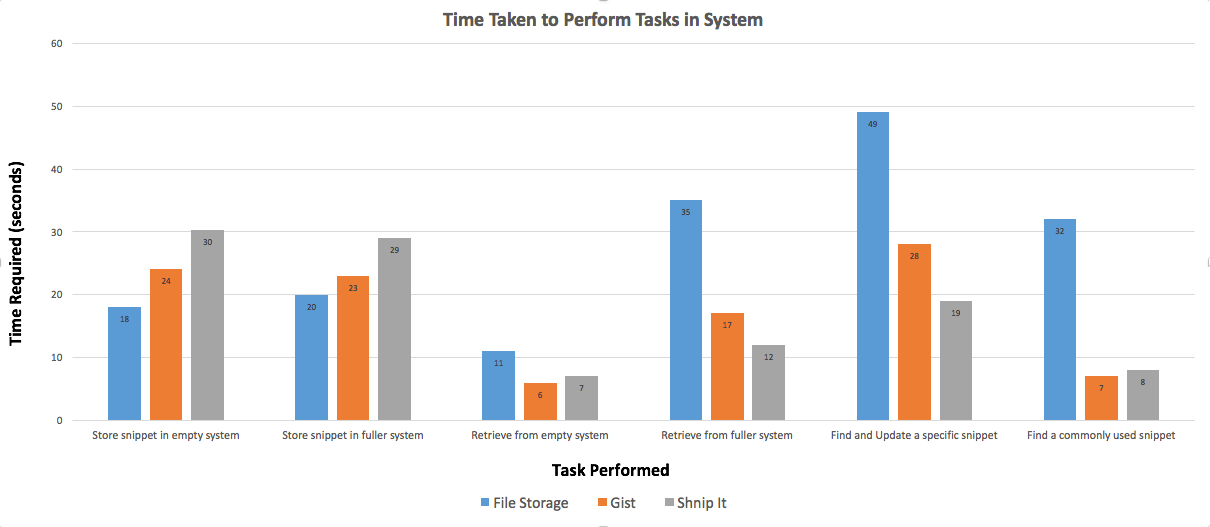
\includegraphics[width=20cm]{SpeedResultsGraph}
\caption{Time taken in seconds per task performed, for each of the 3 systems \label{speedresultsgraph}}
\end{sidewaysfigure}

This graph details the time, in seconds, it takes a user to complete a task, and is measured from the moment the user first interacts with the system, to the moment the final keypress or action button is clicked. 
For retrieval, this includes highlighting and copying the snippet, and for storage this is the action which saves the snippet.
Smaller bars represent a faster system, and as such, the more desireable outcome.

It is interesting to note that, for storage, FS consistently achieved the fastest time, however in all other tasks it was deemed the slowest, and in some cases, by a considerable margin. 
The opposite was true for Gist, scoring slower in storage, but faster in retrieval.
It's clear SI was the slowest in retrieval, and this seemed mostly due to the extra metadata that users had to input, though this then went on to ensure it was much faster than FS for retrieval, and in good competition with Gist, being the fastest for 2 of the 4 retrieval tests, and only a second slower otherwise, on average.

As noted in section \ref{storespeed}, more importance was placed on retrieval, as it's a more common action than storage.
As such, this graph provides a positive outlook on our first goal: that the system is at least on par with current solutions. 

We now look further in-depth into the statistical analysis of our individual tasks, and then go on to provide some insight on observed behaviours gleaned from the screen recordings in section \ref{observationanalysis}.

\subsection{Analysis of Speed by Task}
\subsubsection{Task 1: Storing Snippet within an Empty System}
\begin{table}[H]
\label{speedtabletask1}
\begin{tabular}{ll}
\hline
\textbf{System} & \textbf{Speed (s.d. err)} \\ \hline
FS              & 18 (0.2462)     \\ 
Gist            & 24 (0.4082)     \\ 
SI              & 30 (0.5383)     \\ \hline
\end{tabular}
\end{table}

Mean speed differed statistically significantly between systems. \\
(F = 217.7033, p \textless 0.0001)

Gist speed significantly faster than SI (p \textless 0.001). \\
FS speed significantly faster than SI (p \textless 0.001). \\
FS speed significantly faster than Gist (p \textless 0.001). \\

Not in line with Goal 1 of the system, though this test for storage is less important than retrieval.

\subsubsection{Task 2: Storing Snippet within a Fuller System}
\begin{table}[H]
\label{speedtabletask2}
\begin{tabular}{ll}
\hline
\textbf{System} & \textbf{Speed (s.d. err)} \\ \hline
FS              & 20 (0.2132)     \\ 
Gist            & 23 (0.3257)     \\ 
SI              & 29 (0.2752)     \\ \hline
\end{tabular}
\end{table}

Mean speed differed statistically significantly between systems. \\
(F = 277.2, p \textless 0.0001)

Gist speed significantly faster than SI (p \textless 0.001). \\
FS speed significantly faster than SI (p \textless 0.001). \\
FS speed significantly faster than Gist (p \textless 0.001). \\

Again, not in line with Goal 1 of the system, however, again, this test for storage is less important than retrieval.

\subsubsection{Task 3: Retrieving Snippet from within an Empty System}
\begin{table}[H]
\label{speedtabletask3}
\begin{tabular}{ll}
\hline
\textbf{System} & \textbf{Speed (s.d. err)} \\ \hline
FS              & 11 (0.3128)     \\ 
Gist            & 6 (0.2132)     \\ 
SI              & 7 (0.2843)     \\ \hline
\end{tabular}
\end{table}

Mean speed differed statistically significantly between systems. \\
(F = 102.161, p \textless 0.0001)

Gist speed significantly faster than FS (p \textless 0.001). \\
SI speed significantly faster than FS (p \textless 0.001). \\
Analysis did not show a significant value for SI vs Gist (p = 0.07396). \\

For retrieval in an empty system, Goal 1 is met, as there is no significant difference between Gist and SI, however both systems are significantly faster than FS.

\subsubsection{Task 4: Retrieving Snippet from within a Fuller System}
\begin{table}[H]
\label{speedtabletask4}
\begin{tabular}{ll}
\hline
\textbf{System} & \textbf{Speed (s.d. err)} \\ \hline
FS              & 35 (0.4606)     \\ 
Gist            & 17 (0.5198)     \\ 
SI              & 12 (0.2462)     \\ \hline
\end{tabular}
\end{table}

Mean speed differed statistically significantly between systems. \\
(F = 804.637, p \textless 0.0001)

Gist speed significantly faster than FS (p \textless  0.001). \\
SI speed significantly faster than FS (p \textless  0.001). \\
SI speed significantly faster than Gist (p \textless  0.001). \\

For retrieval in a fuller system, Goal 1 is exceeded, as SI is significantly faster than both other systems.


\subsubsection{Task 5: Finding and Updating a Specific Snippet}
\begin{table}[H]
\label{speedtabletask5}
\begin{tabular}{ll}
\hline
\textbf{System} & \textbf{Speed (s.d. err)} \\ \hline
FS              & 49 (1.3842)     \\ 
Gist            & 28 (0.3693)     \\ 
SI              & 19 (0.4167)     \\ \hline
\end{tabular}
\end{table}

Mean speed differed statistically significantly between systems. \\
(F = 321.72972, p \textless 0.0001)

Gist speed significantly faster than FS (p \textless  0.001). \\
SI speed significantly faster than FS (p \textless  0.001). \\
SI speed significantly faster than Gist (p \textless  0.001). \\

Again, Goal 1 has been exceeded, with SI being significantly faster than both other systems. 
It is interesting to note the large deviation in speeds shown by users of FS, and may relate to the folder structure chosen by the participants, or simply that they struggled to find the specified snippet due to the lack of search functions in FS.

\subsubsection{Task 6: Finding a Commonly Used Snippet}
\begin{table}[H]
\label{speedtabletask6}
\begin{tabular}{ll}
\hline
\textbf{System} & \textbf{Speed (s.d. err)} \\ \hline
FS              & 32 (0.8539)     \\ 
Gist            & 7 (0.1930)     \\ 
SI              & 8 (0.3015)     \\ \hline
\end{tabular}
\end{table}

Mean speed differed statistically significantly between systems. \\
(F = 689.31443, p \textless 0.0001)

Gist speed significantly faster than FS (p \textless  0.001). \\
SI speed significantly faster than FS (p \textless  0.001). \\
Analysis did not show a significant value for SI vs Gist (p = .0168). \\

For this final test of finding a commonly used snippet, Goal 1 is met, as there is no significant difference between Gist and SI, and both systems are significantly faster than FS.
The reason here is that finding a commonly used snippet is mostly identical between the systems, as SI was inspired by Gist, and both utilise a method of specifying a 'starred' snippet for quick retrieval later.


\subsection{Observation of Speed by Task}
Throughout the tasks, number of observations were made regarding the choices the participants made and how the tasks were completed. 
We present them here for consideration in a more qualitative manner.

\subsubsection{Task 1: Storing Snippet within an Empty System}
This task involves using each system in its empty state, with no prior snippets, and simply storing a snippet of code, optionally with metadata.

It was seen that when participants were given a blank folder and a single snippet, they opted not to create any category folders in which to store the snippet, instead opting to simply drop it into the empty folder. 
This meant that FS was quicker than the other two systems, though users seemed to deliberate on how to to store the snippet in the text file, and what metadata to store with it.

Users that utilised the FS as the third system seemed to store more metadata alongside the snippet. 
This may be because they understood what may be useful to store with it, or because they believed it was information the researchers wanted them to store, albeit without being told that.
As such, those users spent longer on the FS than users who utilised it as their first system, where we saw very simple files with minimal information, stored in minimal structure (although this extra time amounted to just a couple of seconds on average).

\subsubsection{Task 2: Storing Snippet within a Fuller System}
This task is mostly similar to the previous one, and similar observations were made.
The speed of task completion is also similar, with slight, single second variances, most likely random and insignifcant in comparison with the previous task.

An interesting observation, however, was that users did spent more time on FS than in the previous task, as now they had to navigate their folder structure, whereas previously, having an empty folder, they would simply create and save a text file.
The extra 2 seconds on average for FS were most likely choosing the folder corresponding to the language of the snippet they were now saving in this system.

\subsubsection{Task 3: Retrieving Snippet from within an Empty System}
In this task, a single snippet was placed within the system, and the users were given information about it and told to retrieve it.
It was the only snippet available within the system, so there was no deliberation over multiple snippets.

Interestingly, despite the users knowing the contents of the system, some users navigated to the wrong folders within the structure, though quickly backed out upon finding no snippet in the folder.
As such, the average time for FS was higher than Gist or SI.

With Gist and SI, the only snippet is immediately available to click on, on the homepage, due to the nature of the systems, and as such allowed users to immediately click it and copy the contents.
This meant they performed faster than FS, though there was no significant difference between the two. 

All users clicked straight through to the snippet, though some took a second or two longer to consider the navigation bar, before realising the snippet was immediately available.

\subsubsection{Task 4: Retrieving Snippet from within a Fuller System}
Within this task is where FS started to struggle, showing its limitations.
Users often clicked through multiple folders, and opened several snippets, before finally finding the snippet they were looking for.
As such the speed of FS greatly drops in this task, and the more complex systems of Gist and SI begin to show their worth.

With Gist and SI, the metadata seemed to play a significant role in expediting the search process for the snippet, allowing users to pinpoint the correct snippet without having to view the contents, or see the actual source code.
This cut down on search time considerably, allowing SI to out perform FS, and even managed to out perform Gist.
It was seen the most likely reason for this is that Gist displays some of the source code along with the snippet, and users seemed to be reading this and taking in more information than with SI, and so slowed down their traversal of the search results.

\subsubsection{Task 5: Finding and Updating a Specific Snippet}
This task began similarly to the previous one, allowing us to again watch users as they retrieved a snippet from a fuller system, though had the added benefit of actioning on a snippet after finding it.

This task had the most variance in time, specifically for FS, as users again struggled to identify the location of the snippet within the folder hierarchy.

Users of Gist and SI found the snippet with much less trouble, making use of the search features and the metadata to find it switfly. 

Editing of the snippet in all systems was relatively simple and understood by all users, with nothing noteworthy to mention.

\subsubsection{Task 6: Finding a Commonly Used Snippet}
At the end of Task 3, users were told to make a mental note of the snippet they added to the system, or to use some functionality of the system they were on, with the knowledge that they would need to navigate back to it many times throughout the test. 
Of course the user did not visit it again until this final task, but it allowed us to instil the the mentality of a commonly used snippet in the user's mind.

Most users used the favourite button on both Gist and SI to save the snippet to a particular location, whereas when using FS, they could only attempt to memorise the location.
As such, FS had a much slower relocation time than Gist and SI, as with the latter, participants could instantly pull up a list containing the snippet. 

One user of SI didn't make use of the favourite button, and instead just searched for the snippet, as in Task 4, which reduced the overall average time by 1 second.
It is unclear whether the user wasn't aware of the favourite function or chose not to use it, however all other 11 participants used the function. 
Further analysis could be done in this area to conclude the reasoning behind this.

\section{Analysis Overview}
This analysis has shown that the first goal of the system has been met: that the system is at least on par with other available systems.
The second goal of the system - that the system enables users to collaborate, ultimately promoting code quality - is yet to be assessed, and will be evaluated via the post-study questionnaire.

\section{Conclusion}
In this chapter we have detailed the results of the quantitative study, as well as perform analysis on them to determine if the first goal of our system has been met.

The next chapter analyses the post-study questionnaire to determine the fate of the second goal, as well as disclose our conclusion on the dissertation and project as a whole.
We also go on to discuss future work available to the system.

 




\chapter{Conclusions, Discussion \& Future Work}
\section{Introduction}
This chapter aims to take the results and their analysis from the previous chapter, and use them to conclude whether the goals, introduced in section \ref{goals} and explained in section \ref{reminderofgoals}, have been met. 
We put forward discussion points for these goals, and use the data collected in the post-study questionnaire to support those points.
Finally, we present conclusions for the dissertation, and discuss opportunities for future work.

\section{Goal Summary}
The evaluation and analysis chapters of this dissertation were present for the purpose of ascertaining whether our two primary goals for the system had been met.
Once again, for the benefit of the reader, those goals were: 

\textbf{Goal 1: To create a snippet repository that is at least on par with existing solutions for storage and retrieval of snippets}. \\
\textbf{Goal 2: To create a system that enables users to collaborate on their saved snippets, to promote quality and keep them up to date}.


\section{Evidence of Goal 1}
The previous chapter presented the analysis of our first goal, and the results are summarised in table \ref{goal1evidence}:

\begin{table}[H]
\caption{Result of Quantitative Tests} \label{goal1evidence}
\begin{tabular}{ll}
\hline
\textbf{Task} & \textbf{Support/Refute Goal 1} \\ \hline
1. Storing in Empty               & Refutes   \\ 
2. Storing in Fuller                & Refutes   \\ 
3. Retrieving from Empty      & Supports \\
4. Retrieving from Fuller       & Supports \\
5. Updating Specific             & Supports \\
6. Finding Commonly Used  & Supports \\ \hline
\end{tabular}
\end{table}

We can see that tasks 1 and 2 refute Goal 1 - that is, Shnip It is not as fast as existing systems in storing the snippet, however this is only a subset of code reuse.
Overall, storing and retrieving the snippet as one action is at least as fast with Shnip It, and considering retrieval is a more common action than storage, it is clear Task 3 and 4 hold more weight than 1 and 2.

The remainder of the tasks all support the goal, and Task 4 and 5 go so far as to exceed the goal, as Shnip It performed faster than existing solutions.

As such, we conclude that Goal 1 has been achieved.

\section{Evidence of Goal 2}
In order to build a case for whether Shnip It has achieved its second goal, the qualitative data gathered from the quantitative study, and its exit questionnaire, are utilised.

For the purpose of this conclusion, the goal is split in to 2 parts: the ability to collaborate, and the effect such collaboration has on code quality.

\subsection{Collaboration}
After completing the 6 tasks, participants had the chance to further examine the system and make use of its collaborative elements, as if they were using it for their own personal use.
The individual collaboration tools were explained to the participants; after that, they were asked to then explore them, before finally completing the post-study questionnaire.

It was seen that participants were confident submitting snippets, and commenting and rating snippets submitted by the other participants. 
Some participants sent push requests to edit snippets owned by other participants, who in turn would discuss them within the confines of the website, and ultimately accept or reject them.
It was seen that even in such a test environment with a small set of users, collaboration was possible and present.

One participant noted that ``\textit{the comments are useful for discussing parts of the code, without having to get too involved in writing}'', which suggests participants can quickly contribute their collaborative opinions and provide thoughtful discussion without even writing code.
Furthermore, being able to submit edit requests ``\textit{allowed me [sic] to get hands on and show what I think the correct code looks like}'', which provides an obviously collaborative environment for user interaction, allowing code snippets to progress through multiple stages, rather than being written, saved and forgotten.

When asked if the tools designed for collaboration were adequate, one participant reported ``\textit{there is a good range of ways to interact with the code, like rating the snips [sic] to show which are good, or asking questions about them in the comments to help me understand them}''. 
This supports the idea that the tools work as they should and that users find them useful and fit for purpose. 

However, it was also mentioned that ``\textit{I [sic] saw long conversations that were off-topic, but no obvious way of dealing with or moderating them}''. 
This quote relates to how there is no approval for comments, and that anyone with an account is able to write anything.
It highlights an important aspect, and as such will be discussed in section \ref{futurework} Future Work.
For now, we believe Stack Overflow has an implementation of comments that potentially would work well on Shnip It, and as such, this would be our first point of research when developing them further.

As a result of this analysis, we conclude that the system does allow for collaboration between users, and that the tools provided for collaboration are fit for purpose.

\subsection{Promoting Quality Code}
One important question still needs to be address: can the collaboration techniques employed be utilised to increase the quality of the reuseable code, and also keep the snippets up to date.

As a test for this, before letting the participants loose on the system, 3 snippets were artificially inserted in the system and given a high rating so they would appear in the top snippets.
However these snippets were either out of date or incorrect.
It was our desire that, upon exploring and interacting with the collaborative elements of the system, the participants would discover these artificial snippets, and either discuss them, or ultimately change and update them to improve them.

We saw both discussion and edits being made to all 3 of the snippets, meaning that, with just a group of 12 users, the faulty code was being reviewed and modified, ultimately improving the quality of the code.

One participant commented: ``\textit{I found some code that was wrong, but I didn't wanna [sic] change it. Instead I put a comment, and then some other guys commented too agreeing with me, so I ended up submitting an edit request, which was approved}''.
This participant found one of the artificial snippets and realised it was incorrect, but was put off from changing it due to the high rating it had already accrued. 
Instead of ignoring it, he left a comment with his opinions on what he thought was incorrect about it.
Several other participants did the same thing, creating a conversation that ultimately ended in the participant changing the code and submitting an edit request, which was accepted, and the snippet was now improved.

This shows that the collaborative techniques do promote quality code, as they were utilised to take an incorrect snippet of code, build a dialogue around it, and finally output a correct snippet of code.

A similar scenario was seen with the out of date code, where a conversation formed around a piece of code that stated it was only for an older version of PHP.
Participants discussed it, and decided they wanted to preserve the old PHP code, but have the new PHP code too.
The initial edit request contained both pieces of code within the same snippet.
Interestingly, further conversation around the snippet provoked a second edit request to be submitted, which actually turned the snippet into a collection, and the snippet for the new version of PHP was submitted as a separate snippet within the collection.

Such a scenario demonstrates an eco-system forming within Shnip It, amongst even just 12 users, where they collectively negotiate and decide the best course of action for a particular snippet. 

As such, there is good evidence to suggest that the system's collaborative techniques tend to promote code quality; there is also evidence to suggest that it provides a method of keeping that code up to date.

Based on the analysis of this section, Goal 2 has been met.

\section{Participant's Opinions}
The post-study questionnaire gathered a number of opinions from participants, which are presented within this section.

Upon being asked which of the systems the participants preferred, 11 of 12 chose Shnip It as their preferred system for code reuse.
One participant selected Gist, and left a comment saying that this is the tool they are used to already, and that they work frequently with GitHub, which integrates with Gist.
It was noted that the participant would consider Shnip It if it integrated similarly with GitHub to automatically create a repository from the snippet.

Participants felt that the length of time taken to store and reuse the code was reasonable for Shnip It and Gist, and unreasonable for the File System, and all participants chose Yes, when asked if they thought Shnip It was at least as fast as the other systems.

Shnip It was rated as highly easy to use, averaging a higher score than Gist and a significantly higher score than the file system.
Furthermore the collaborative elements were decidedly rated as Highly Useful, and all participants chose Yes, when asked if they thought it helped promote quality code.

The opinions of the participants are in line with the goals of the system, and as such further cement our conclusion that the goals of the system have been met.

\section{Summary} \label{conclusionsummary}
\subsection{Goal 1: Speed}
The analysis found that the system meets our first goal of being as efficient as the existing systems we tested, and in some scenarios that speed was even improved by Shnip It. 
As a result, the first goal of our system has been achieved.

\subsection{Goal 2: Collaboration}
It was witnessed, and reported by participants, that the system provided appropriate tools for collaboration, and that such collaboration was beneficial for the quality of the code, and its relevancy.
As such, the second goal of our system has been achieved.

\subsection{Participant Opinion}
Participants of the system decidedly chose Shnip It as the most preferred system, citing it at easy to use, and agreeing that it was both as fas as the existing systems tested, and that the collaboration elements were present, and useful for improving the quality of code.
This feedback reinforces the conclusion that both goals of the system have been met.

\section{Conclusions}
We conclude that Shnip It has met the requirements and goals set out before it, and as such, demonstrated that a collaborative snippet repository can be created.

We summarise the journey taken here, and the criteria and goals achieved:

\subsection{Initial Research Criteria}
We began with the initial criteria identified for the project, from section \ref{probdesc}, excluding out of scope search and sort:
\begin{itemize}
\item The developer may not reuse at all, and so waste time rewriting code.
\item The developer may not update code in line with language advancements, leading to stale code. 
\item The reusable code may have a lack of peer review in a personal or limited use repository.
\item Maintaining/modifying the repository itself in response to the evolving needs of the software developer(s). 
\end{itemize}

The overall project addresses the first point.
The collaborative elements address the second and third points.
The final point is addressed in section \ref{evolvewithneeds}, where we discussed maintaining the repository, and its evolution.

\subsection{System Goals}
In section \ref{goals} we identified 2 main goals for the system, of which we aimed our proposed system to meet: \\
\textbf{Goal 1: To create a snippet repository that is at least on par with existing solutions for storage and retrieval of snippets}. \\
\textbf{Goal 2: To create a system that enables users to collaborate on their saved snippets, to promote quality and keep them up to date}.

\subsection{Requirements}
We specified the requirements in section \ref{requirements}, and detailed how the system had met those requirements in section \ref{requirementsrevisited}.

We noted that all high priority requirements, both Functional and Non-Functional, were met, with the exception of complex search and sort, due to the nature of scope of the dissertation.
However, several of the Non-Functional requirements were left for evaluation during the Usability Study.
We also noted that of our 3 low priority requirements, we completed just 1, due to time constraints on the system, but we leave the remaining two for future work (\ref{opensource} Open Source and \ref{gamification} Gamification).

\subsection{Evaluative Studies}
\subsubsection{Usability Study}
During this Usability Study, we evaluted several of the Non-Functional requirements that required a first time user, such as \ref{easeofuse} Ease of Use and \ref{simpleandclear} Simple and Clear.
The full transcript of the study can be found in Appendix \ref{appendixusabilitystudy}.

\subsubsection{Quantitative Study}
From our Quantitative Study we evaluated 5 questions, found in section \ref{overallgoals}, which were geared around solving our two main goals of the system.
As such, we evaluted the study with these 5 questions in mind, before performing analysis on them.

\subsection{Analysis and Conclusion}
Finally, we completed analysis of our studies, and concluded that both goals for the system were met, and that the majority of participants preferred Shnip It over the tested alternatives.

Our system is openly accessible to anyone with an internet connection and a web browser, with no barriers to entry for viewing, and a minimal barrier for contribution: simply, account creation. 
We feel that the system has demonstrated its validity via the participant opinion questionnaire, and having mets its goals, we feel it could become a beneficial platform for collaborative code reuse.


\section{Future Work} \label{futurework}
Shnip It works as intended, with many features implemented, allowing full use of the system.
Despite this, there are a number of ways we could improve our system, and further research to be performed.

Initially, the two low priority requirements that were not met could be explored.
\begin{itemize}
\item Make the code available via Open Source, and allow further collaboration on the system itself, by opening it to public code edit requests.
\item Provide gamification elements to the website to promote positive use and repeat interaction, such as achievements for positively interacting with the website or points for having your snippets upvoted.
\end{itemize}

The system could be refined in areas:
\begin{itemize}
\item The comments section could be improved, taking inspiration from Stack Overflow, to relocate long conversations and prevent spam.
\item Ensuring the system is fully compatible in all browsers, across all devices, including computer, phone and tablet. Furthermore, making the website look good even in older, incompatible browsers.
\end{itemize}

Further features worth considering:
\begin{itemize}
\item Further uses in Education - enabling students to submit code for a lecturer to review and critique, or providing a collaborative learning environment within the website.
\item Providing interaction with GitHub to create a git repository straight from a snippet, as mentioned by a study participant.
\item Exposing an API to allow IDEs to hook into the user's account and pull a list of snippets for instant use in the code editor.
\end{itemize}

Further research can be performed:
\begin{itemize}
\item Specifically on the problem of Search and Sort, and creating a well rounded algorithm for it
\item Research into algorithms to display the most appropriate snippets on the homepage, via rating over time over interaction, etc.
\end{itemize}

And further studies can also be performed:
\begin{itemize}
\item Evaluate how snippet collections should be rated - individually for each snippet in the collection, or collectively for the entire collection.
\item Further usability studies, as originally intended, to class a broader range of users into the analysis.
\end{itemize}


It is clear there are a variety of ways to further work on the system, and it is likely the author of this dissertation will continue to do so.
It is clear Shnip It can contribute to the state of code reuse, even if just on a small scale, and ultimately help developers increase both the reusability, and the quality, of their code, raising overall standards of all users.
It is an exciting prospect to continue development on the project into the future.






\bibliography{BibFile}


\appendix

%%
%% Use the appendix for major chunks of detailed work, such as these. Tailor
%% these to your own requirements
%%

\chapter{Usability Study}

\section{Tasks Performed} \label{usabilitystudytasks}
\begin{itemize}
\item \textbf{Task 1}: Find a HTML5 template snippet
\item \textbf{Task 2}: Store some specific code in a new public snippet
\item \textbf{Task 3}: Find a previously written snippet, update its title and set it to public
\item \textbf{Task 4}: Find a PHP snippet that's outdated, turn it into a collection and add an updated version to it
\item \textbf{Task 5}: Find a snippet you changed earlier, and revert the changes
\item \textbf{Task 6}: Perform interaction with snippets, including commenting, rating and edit requests
\end{itemize}

\section{Study Transcript} \label{usabilitystudytrans}

\begin{lstlisting}[caption={Transcription of Usability Study}]
\end{lstlisting}
J: Researcher (Jamie) \\
P: Participant

*The participant has the aim and deliverable of this dissertation explained to them. The computer in front has an open browser, with Shnip It open in the browser.*

J: \-\hspace{1.4cm} So let’s start by getting a feel of reusing code as a new user. Try to find a code snippet for a HTML5 document template. \\
P: Okay. \\
P: I can’t see any HTML snippets on the homepage, they look to be CSS and java mostly. I’ll click up here and search for it.  \\
P: *Clicks in search bar* \\
( Participant is able to quickly digest snippet information, including what language each snippet is, without having seen it before. )

P: *Types HTML5 boilerplate*  \\
*Page refreshes with search results*  \\
P: So this first one is called Cheeky HTML 5 boilerplate, and has more upvotes than any of the ones below it, so I'll pick this one. \\
P: *Click the name of the snippet* \\
( Expert performance, with no prompting. Understood snippet meta data, searching and accessing the snippet, immediately. )

*The snippet page opens to display the snippet*

P: Oh I like that the description looks like a html comment. Does that happen for each language? \\
J: \-\hspace{1.4cm}No, it's entered by the user when they type the snippet, so it can just be text. \\
P: You could definitely code that yourself! 

J: \-\hspace{1.4cm}Okay now you can find snippets, let's try adding your own one. Here's some code that you want to store  \\
J: \-\hspace{1.4cm}*Points to a wordpad file open on the computer*.  \\
J: \-\hspace{1.4cm}Try to create a snippet with appropriate meta data, that's public for everyone to use. \\
P: Okay so there's a create button in the navbar  \\
P: *Clicks create, then clicks A Snippet*.  \\
*The login page appears* \\
P: Oh I need to login first. Do you have a test account I can use or should I make one? \\
( For the purpose of this study being quick, the researcher logs in using a pre-existing account )

*The create snippet page appears*

P: I like that login screen, the bar of colours looks nice. \\
P: Okay so, first I can set the language, so this snippet looks like CSS to me, yeah? \\
J: \-\hspace{1.4cm}Yeah \\
P: So I'll select CSS. What happens if I want to store a snippet that- oh there's an Other selection. So you could pick that if it's not supported? Cool.  \\
P: Then I'll enter some tag words. 
P: *Types a few key words (background, color, gradient)*  \\
P: *Types a title (Set background colour gradient)* \\
P: So in the description, I have to write the comment tags myself to make it look nice on the snippet? \\
J: \-\hspace{1.4cm}Yep, they're not automatic \\
P: Okay so I'll put those in  \\
P: *Types a description, inside of /* and */ tags* \\
P: And finally the snippet goes here  \\
P: *Pastes snippet, and clicks Create Public Snippet* \\
( Expert performance again, easily finding the create section and submitting the snippet. ) \\
*The snippet is created and displayed on screen*

J: \-\hspace{1.4cm}Okay great, well done! So now, let's say you've decided a previous snippet you've written needs to be updated, and then needs setting to public. Try to find the private snippet called 'Not a good snippet', and change it to 'Good Snippet', and set it public. And don't use the search bar for this bit either. \\
P: Find it? Okay so there's a place called Boards, I'm guessing that's like a collection of snippets.  \\
( User understands the terminology of the site without it being mentioned to them ) \\
P: I'll go there and see if mine are in there. I don't know where I'm looking though.  \\
P: *Clicks Boards in the navigation bar. More options appear.* \\
P: *Clicks My Boards* \\
*A list of the user's boards appear* \\
P: So there's quite a lot of boards here, I'm not sure where to start without the search bar. Is there a way to search through this My Boards page? \\
J: \-\hspace{1.4cm}No but I like that idea, I think that's good to limit the search to specific spaces. However, advanced search and sort will come later in the project as it's not in the scope of my dissertation. \\
P: Okay, so do I just need to go through them all? \\
J: \-\hspace{1.4cm}Try going to your profile page. \\
P: Profile page... So up here  \\
P: *Clicks on account name, then on View Profile* \\
*The user's profile page opens* \\
P: So there's some snippets on the right, I'm guessing I should click View All... *Clicks View All* \\
*The page changes to show all the user's snippets, sorted by most recent updated date* \\
P: And then there's two pages of snippets, so that's easier.  \\
P: *Presses Ctrl + F, types Not a, and then clicks on the 'Not a Good Snippet'* \\
*The appropriate snippet page is displayed on screen* \\
P: Got it! \\
( We hadn't been to the profile page yet, but once there, the user understood immediately that they could view all of their snippets from there. )

P: So I need to change the title, and the visibility setting to public? \\
P: *Clicks pencil icon for edit* \\
*The edit snippet page is displayed* \\
( No prompting here! User understands the function icons and what they will do ) \\
P: *Changes the title as requested, and sets the snippet to public* \\
( Again no prompting on this page! It closely resembles the Create Snippet page in layout and design, and this is seen by the expert performance demonstrated! ) \\
P: Okay, I think that's that. Just the title and the publicity setting? \\
J: \-\hspace{1.4cm}Yep, that's it! Perfect. \\
P: *Clicks save snippets* \\
*The snippet page is displayed again*

J: \-\hspace{1.4cm}So let's do something a bit more complex now - there's a public PHP snippet called 'Access Database', but it's written in PHP 5. We want to change it to PHP 7, without overriding the existing snippet. I want you to find the snippet, then turn it into a Collection, and add a second snippet to it, the PHP 7 one. \\
P: What's a collection? \\
J: \-\hspace{1.4cm}It's where one 'snippet', so to speak, actually holds multiple snippets, like a snippet for a button might have html, css and javascript. \\
P: Okay I see. \\
P: *Clicks Boards > Public Boards* \\
*List of public boards is displayed* \\
( User seems to be under the impression that we still don't want them to use the search bar, which suits our needs fine ) \\
( User immediately understands where to find the snippet, without having been there before, due to the Boards > My Boards ) \\
J: \-\hspace{1.4cm}What made you click here? \\
P: You said it was public, and I'm not using the search bar, so I figured I would find it here. I'm guessing it's in this PHP board here \\
P: *Clicks to open the PHP board* \\
*The PHP board is displayed on screen, showing some of the snippets* \\
P: *Presses Ctrl + f to find Access Database, and clicks the title* \\
*The snippet is now displayed on screen* \\
P: Um, oh yeah okay this is it. Yeah I thought this wasn't PHP 5 but it is. Do you want me to write one in 7? Or do you have another one? \\
J: \-\hspace{1.4cm}Yeah I have one *Points to another wordpad file* \\
P: Okay so, I click Edit snippet, and then Create Collection? \\
J: \-\hspace{1.4cm}Yep \\
P: *Clicks Create Collection* \\
*The edit snippet page changes to show it's now in a collection, and extra options appear* \\
P: And so now I have a snippet in the collection so I need to add another one  \\
P: *Clicks the + button to add another snippet* \\
( User immediately grasps the concept of Collections and how to build them from snippets ) \\
P: Which wordpad file was it? \\
J: \-\hspace{1.4cm}*Points to the file* This one \\
P: Okay thanks, so I'll paste all this in to the new boxes. It's good because it's all the same fields and same layout and everything so it seems quite easy to make more snippets. I'd get used to this quite quickly. Just need better searching so I can find things faster. \\
J: \-\hspace{1.4cm}Yeah, like I said that will come in the future, otherwise it's too much for one dissertation. \\

................ 

P: *Enters the rest of the snippet detail then hits save* \\
*Page changes to view the snippet, with a message saying it's awaiting confirmation, and a message explaining why* \\
P: Okay, I've added the PHP 7.0 one. It says that it's awaiting confirmation. \\
J: \-\hspace{1.4cm}Yeah so there's two ways for this to be  added - either the original author accepts the change request he just received, or the community vote it positively past a threshold. Currently that threshold is 20 positive votes, but the plan is to make it dynamic based on current and historical data trends, and user weightings. Unfortunately, again, that's out of scope for the system at the moment. \\
P: Great so, if the user accepts it, it just changes? Can it go back? \\
J: \-\hspace{1.4cm}Yeah, all snippets have complete version history and control. 

J: \-\hspace{1.4cm}So while we're on that topic, lets go back and revert the 'Good Snippet' back to the previous 'Not a good snippet', making sure it's private again. \\
P: Okay. *Clicks on profile, finds snippet, clicks for version history* \\
( User is able to easily remember and recall previous actions like an expert user, and navigates perfectly and efficiently. ) \\
*The snippet is displayed, then the history of the snippet is displayed as a timeline* \\
P: Oh so there's a timeline a bit like github, or stack overflow. You should have diff to show exactly what changed. \\
P: *Clicks the restore snippet button*. \\
P: And so that's it. Does it save the 'Good Snippet' now in the version history? \\
( User intuitively navigates and interacts with the version control without prompting or prior knowledge! ) \\
J: \-\hspace{1.4cm}Yeah, it makes a new record. I've toyed with just moving the order when you restore, or deleting the HEAD up to that snippet, but I think this way is more complete, though it might need some maintenance for long history snippets. I might add an option to delete history, or hide from the main listing or something like that.

J: \-\hspace{1.4cm}Finally, lets do some interaction. From the homepage, take a look through some of the snippets and use the interaction functions to express your opinions. \\
P: Interaction functions? \\
J: \-\hspace{1.4cm}Like leaving a comment, favouriting a snippet, rati- \\
P: Ah okay I see what you mean.  \\
J: \-\hspace{1.4cm}-ting a snippet. \\
P: *Clicks Shnip It logo to go to homepage* \\
*Home page appears* \\
P: I'll just read a few then and react as I would do. \\
P: *Participant begins going through snippets, and voting them up or down and commenting why. The participant submitted an edit request for one too* \\
( All interaction was unprompted, and the participant clearly understood what he was doing, without making any mistakes. )

J: \-\hspace{1.4cm}Okay I think that's enough, thanks. 

---------------

J: \-\hspace{1.4cm}So that's all of the test cases, so thank you for your time! \\
P: Yeah no worries, it looks good \\
J: \-\hspace{1.4cm}So I just have a few questions if you wouldn't mind answering them. \\
P: That's fine, go ahead 

J: \-\hspace{1.4cm}Okay, so, first of all, what are your first impressions of the system? What are your thoughts? \\
P: Well it seems to do what it sets out to do, albeit it needs more search to be complete, but I know you have that on the roadmap. It looks clean which is good, and although each snippet has a lot of information, it's clearly laid out and well styled to differentiate the data. \\
I wonder how you will sort the 'popular' snippets on the homepage, as right now it looks like they're just being chosen based on the most votes, which would lead to the most popular snippets being permanently sorted to the top with nothing else able to reach it. Though I suppose that may be desireable. I'll let you work that one out! \\
Overall I quite like it and would like to follow its development.

J: \-\hspace{1.4cm}Did you feel comfortable using the system without prompting? \\
P: Yeah I don't think you prompted me very much, other than with going to the profile page, but I couldn't use the search bar so that makes sense. For the most part, it was quite obvious what each part of the system was going to do.  \\
J: \-\hspace{1.4cm}Can you expand on what you mean by how the parts were obvious? \\
P: So like, the call to action buttons did what I thought they would do, because the text and icons on those are similar to other website's that I've used. I didn't have to guess much since it's a similar feel to other systems.  \\
J: \-\hspace{1.4cm}And did you feel it was quite simple and clear, or did it feel cluttered or busy? \\
P: Yeah I like the layout and the design, it didn't feel like there was too much or anything. There's a lot of information on the snippet when they're in a list, but the styling on the text makes it easy to distinguish what each piece of data is, and you use colour well to emphasize the important bits, so I would say yeah overall it is simple and clear. 


J: \-\hspace{1.4cm}Do you feel the system is suitable for small scale developers to utilise for code reuse? \\
P: Yes I think it would be, as it would allow a central repository for common, uh, snippets. I wonder if splitting it into different sub-websites, like Stack Overflow has done, for example one for web developers, one for other mediums etc, but I don't know the scope of that. You could also include other files like common designs, say for UML diagrams, or README files and things like that rather than just code. \\
I think it would be good for web developers though, for sure, I really like it, especially the collaboration part of it, if it works well.

J: \-\hspace{1.4cm}And how do you feel then about using it with your company to share and reuse code, such as having several private boards for your colleagues to use? \\
P: So like giving each team a board, and then giving all employees access to their team boards, or even access to all the boards? I think it would work quite well, but I wouldn't want to have to navigate through all the public stuff as well. I would want it to be maybe switched into a company mode, maybe -company name redacted-.shnip.it as the URL, then all the searching is just within that companies assets etc. But I think it would work well company wide too. Perhaps without the rating system though, I don't know if that's good or bad in a workplace environment. You might need to look in to that at a deeper level.


J: \-\hspace{1.4cm}Do you feel having the collaborative elements of the website would help keep the code updated with language advancements? \\
P: So this is like in reference to the PHP 7 snippet that we did? Yeah I think it's something I've found annoying when I've had to switch to a new branch of PHP, and I sort of just start a new snippet collection because I don't have the time to go through and update them all. If people contribute to this and we have a central repository of generic snippets in the different code versions, yeah I think that's something that the website could do well. It certainly won't harm the ability to keep the code updated, but I think maybe some sort of moderation would be required, similar to Stack Overflow - maybe power users that are given extra power to moderate submissions, like a community to govern the community.

J: \-\hspace{1.4cm}And did you feel the collaborative elements of the website made it better than conventional storage systems?
P: I think the trade off for having the collaborativity is the loss of a personal storage - it's now shared with others, and with that brings other coding stylings and opinions. That being said, you're not removing the personal storage element as you have your private boards, so it's more like choosing which route you want to go down.  \\
P: So yeah I would say it is better than the conventional storage, as you can choose to have the simple, personal boards, or to contribute and collaborate with the wider community, which lowers your workload considerably, expands your options and provides you with, what I assume you'll strive for, the best possible code snippets.

J: \-\hspace{1.4cm}Do you think such a system would increase the quality of reuseable code throughout the community in comparison with a non-collaborative system? \\
P: Stack Overflow is usually good at weeding out the bad answers and highlighting the good answers, at least in my experience, but any sort of collaborative system is only going to be as good as its users. I think the idea of super users as moderators, who have shown their expertise, would be the key to keeping the quality of the reuseable code high, but the best coder in the world is always going to produce a better personal code repository than 500 users all new to programming.  \\
P: I think, therefore, providing some form of moderation is the key to how successful this quality element of collaboration is, and also being able to grab and keep the attention of good programmers, and fold them into the community, is what will make it good. So yeah, providing you can attract and retain those expert level programmers, I think it will increase the quality of reuseable code.

J: \-\hspace{1.4cm}Great, thank you, that's all of my questions \\
P: Okay cool. Oh send me a link to this too, I want to keep an eye on it. \\
J: \-\hspace{1.4cm}Yeah for sure, I'll email you when it goes live

...............


 \label{appendixusabilitystudy}

\chapter{Quantitative Study}

\section{Participants General Information}
\begin{figure}[H]
\centering
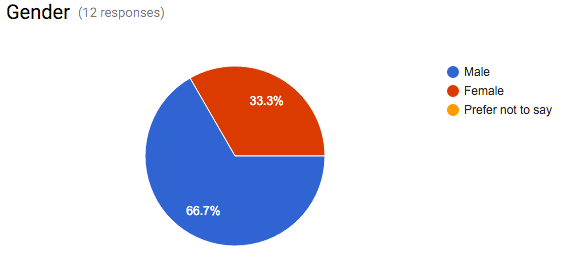
\includegraphics[width=13cm]{genderpie}
\caption{Pie Chart of Participants Gender \label{genderpie}}
\end{figure}



\begin{table}[H]
\centering
\caption{Participants Ages \label{agetable}}
\begin{tabular}{llllll}
\hline
  & Count & Min & Max & Mean & Std. Dev \\ \hline
Age  & 12 & 18 & 25 & 21.33 & 2.57  \\ \hline
\end{tabular}
\end{table}


\section{Previous Experience}

\begin{figure}[H]
\centering
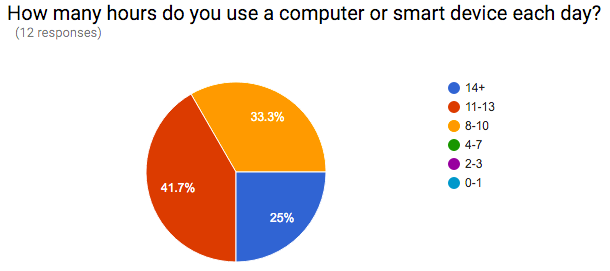
\includegraphics[width=13cm]{deviceusage}
\caption{Pie Chart of Participants Device Usage \label{deviceusage}}
\end{figure}

\begin{figure}[H]
\centering
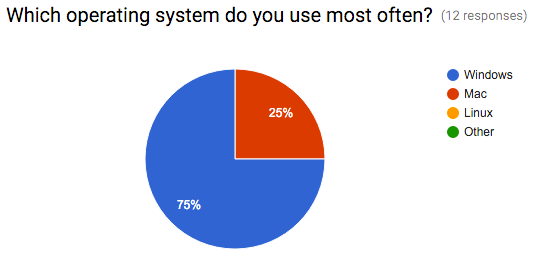
\includegraphics[width=13cm]{osusage}
\caption{Pie Chart of Participants Operating System Usage \label{osusage}}
\end{figure}

\begin{figure}[H]
\centering
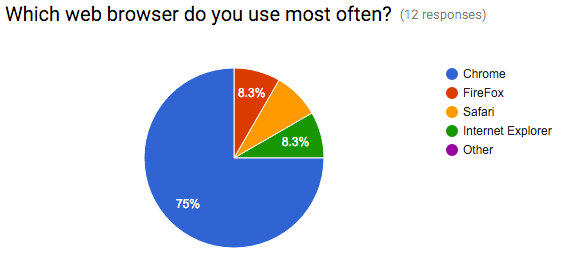
\includegraphics[width=13cm]{webbrowserusage}
\caption{Pie Chart of Participants Browser Usage \label{webbrowserusage}}
\end{figure}

\section{Code Reuse}

\begin{figure}[H]
\centering
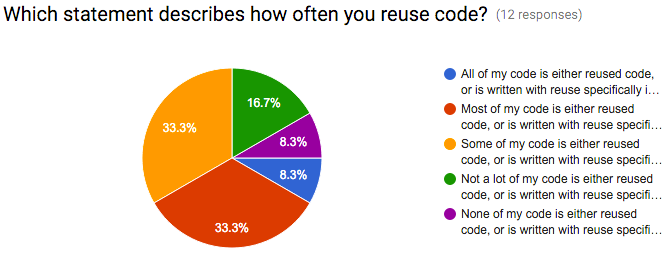
\includegraphics[width=13cm]{codereuseoften}
\caption{Pie Chart of Participants Current Code Reuse \label{codereuseoften}}
\end{figure}

\begin{figure}[H]
\centering
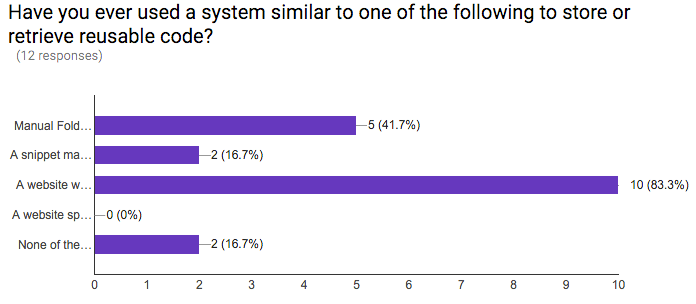
\includegraphics[width=13cm]{systemusebarchart}
\caption{Bar Chart of Participants Experience with Existing Systems \label{systemusebarchart}}
\end{figure}

\section{Initial Questionnaire} \label{appendixquestionnaires}

\begin{figure}[H]
  \centering
  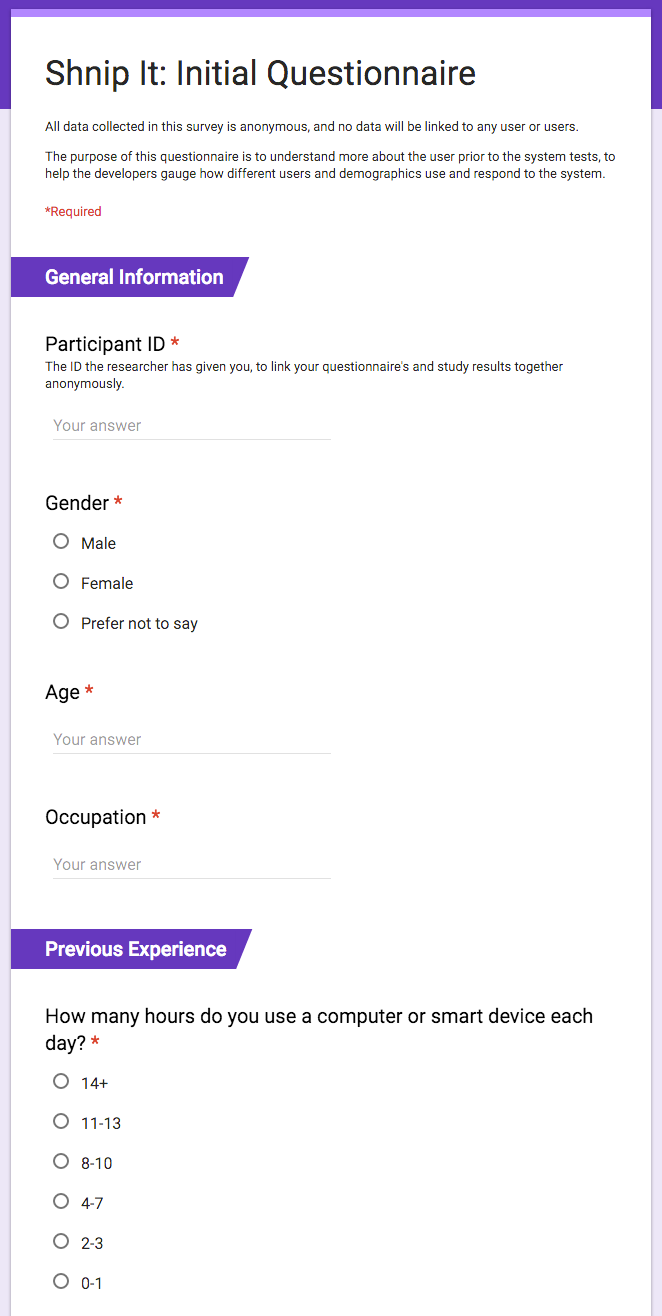
\includegraphics[width=10cm]{firstquest1}
  \caption{Initial Questionnaire \label{initialquestionnaire}}
\end{figure}

\begin{figure}[H]
  \ContinuedFloat
  \captionsetup{list=off,format=cont}
  \centering
  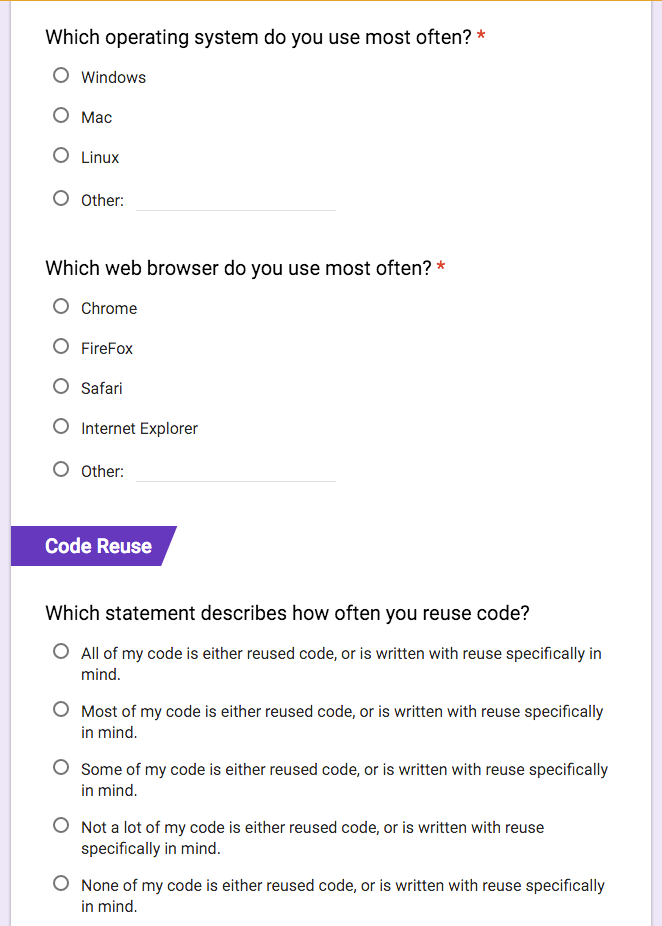
\includegraphics[width=10cm]{firstquest2}
  \caption{First figure continued}
\end{figure}

\begin{figure}[H]
  \ContinuedFloat
  \captionsetup{list=off,format=cont}
  \centering
  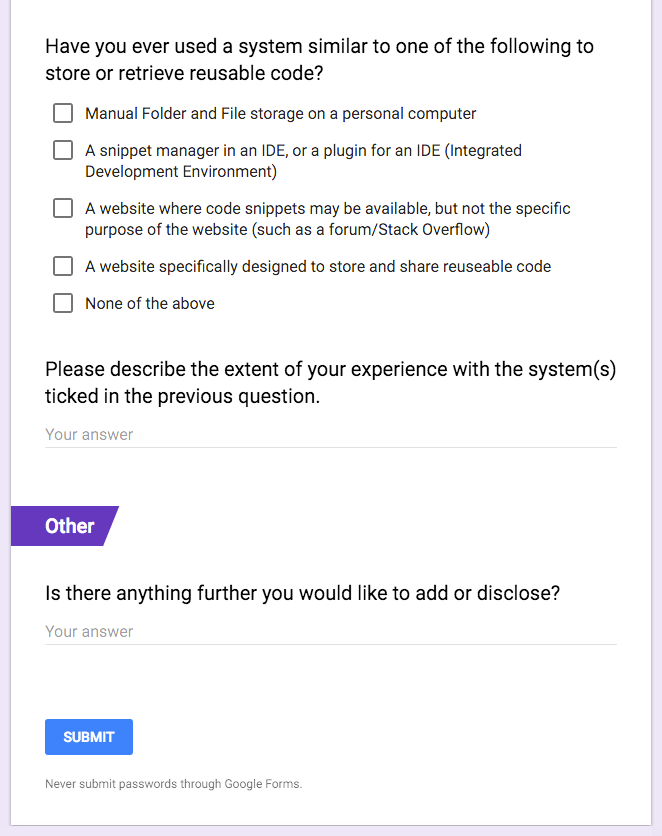
\includegraphics[width=10cm]{firstquest3}
  \caption{First figure continued}
\end{figure}

\section{Permission Slips} \label{appendixpermission}
\begin{figure}[H]
  \centering
  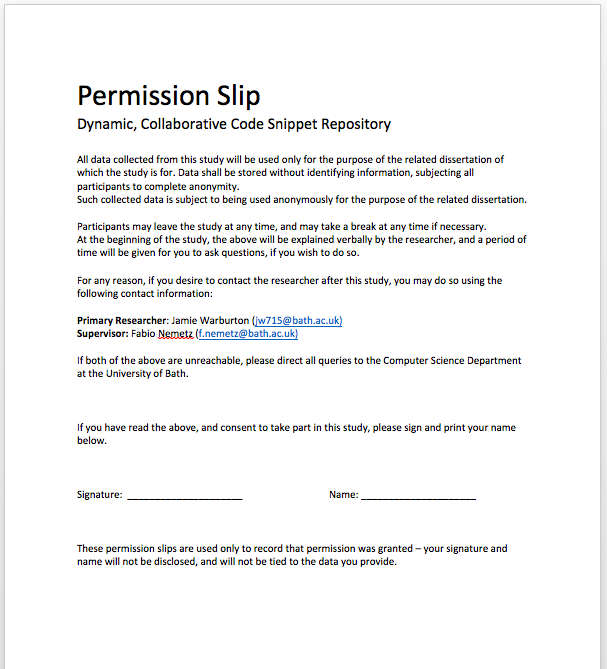
\includegraphics[width=13cm]{permissionslip}
  \caption{Study Permission Slip \label{permissionslip}}
\end{figure}





\chapter{Code Excerpts}

\begin{landscape}
\begin{multicols}{2}
\section{Medoo} \label{medoocode}
\lstinputlisting[frame=single,basicstyle=\scriptsize,language=PHP,caption=Insert into Database]{code/medooaccess.php}
\end{multicols}
\end{landscape}

\begin{landscape}
\begin{multicols}{2}
\section{Generic Functions} \label{snippetgrab}
\lstinputlisting[frame=single,basicstyle=\scriptsize,language=PHP,caption=Generic Snippet Pull from Database]{code/snippetgrab.php}
\end{multicols}
\end{landscape}

%%
%% NOTE that for this to typeset correctly, ensure you use the pdflatex
%%      command in preference to the latex command.  If you do not have
%%      the pdflatex command, you will need to remove the landscape and
%%      multicols tags and just make do with single column listing output
%%

%%\begin{landscape}
%%\begin{multicols}{2}
%%\section{File: yourCodeFile.java}
%%\lstinputlisting[basicstyle=\scriptsize]{yourCodeFile.java}
%%\end{multicols}
%%\end{landscape}

\end{document}
